\documentclass[12pt]{UoAthesis} \usepackage{booktabs}
\usepackage{color} \usepackage{graphics} \usepackage{enumerate}

\thesistitle{The Development of a General Method to Map between
  Continuous and Discrete Molecular Potentials}
\thesisauthor{Christopher James Thomson} \thesispdfkeywords{}
\thesisyear{2012}

\thesisabstract{Molecular interactions are frequently described using
  either continuous or discrete intermolecular potentials.  The
  objective of this dissertation is to develop a general technique for
  converting continuous molecular models to discrete
  forms. Discrete models have many desirable properties; they allow
  the use of event-driven molecular dynamics, which is more accurate
  and stable than traditional techniques.  Discrete potentials also
  have a set of well-developed theories allowing accurate predictions
  of the equations of state and transport properties.

  An event-driven and a force-driven simulator are developed for this
  dissertation to test the effectiveness of number of proposed
  conversion methods.  A novel technique is proposed, which appears to
  accurately reproduce the thermodynamics of the original continuous
  potentials. This technique opens the door to rapid and accurate
  predictions of thermophysical properties from existing
  molecular interactions found in the literature. }

\acknowledgements{Firstly, I would like to thank my supervisor
  Dr. Marcus Bannerman for introducing me to the world of molecular
  dynamics.  Without his seemingly infinite amounts of patience,
  enthusiasm and wisdom, this dissertation would not have been possible.

  I would like to thank my family for their continual support, and for
  donating their computers which allowed me to run the many
  simulations required to complete this project.  I would also like to
  thank my father for taking the time to help proof-read this
  dissertation.}

%%% The bibtex file where your references are stored 
\bibliography{main}
\begin{document}

%%% = = = DISSERTATION OVERVIEW = = =

% - INTRODUCTION - %
% Molecules, why are we interested in the molecular scale? What processes are molecular
% - - Molecular dynamics, what is it, why is it important to Chemical
%engineering.

% - - Leading into potentials, need for faster methods, more accurate methods.%
%Review of existing literature (Chapela, PRIME SPEADMD), what they've done,
%why its not as good as what you're going to do % 

% Outline of the thesis to come

% - Molecular Simulation 
% -- Newtonian mechanics F=MA, is it valid? 
% -- Forces from potentials (conservative forces) 
% Types of forces (gravitational (which is neglected)), pairwise forces 
% leading to intermolecular potentials.

% --- Give an example soft potential (LJ), Introduce a discrete -- 
% -potential,hard sphere is the prototypical discrete potential, -- 
% -but there are stepped potentials too (Chapela). Talk about the -- 
% -advantages/disadvantages etc.

%%%% Lead out of the chapter with this 
% --- Introduce discrete potentials, say they need a special method of solution
%(EDMD).
% - Simulation Methods - % 
% - -Force Driven Simulators 
% - - - Introduction and general algorithm 
% - - -Integrators: Euler, Verlet, Velocity Verlet, Gear...lit review to find
%more recent ones
% - - - Optimization: neighbour lists, truncation of the potential 
%- - - Adv/Disadv? or just within other relevant topics 
% - - Event Driven Simulators % - - - Introduction and general algorithm 
% - - - Collision rules 
%Actually older than force based, although not as popular.
% - - - Optimization: neighbour lists, O(1) priority queue algorithms, time warp%algorithms
% - -Measuring System Properties % - - - Radial Distribution Function
 % - - -Temperature 
% - - - Pressure 
% - - - Coefficient of Diffusion 
% - Results - % 
 % - Discussion- % 
% - Conclusions - % 
% - Recommendations for future work - % 
% - Appendices -% 
% - - Derivation of collision rule for stepped potentials %
%% = = = END OVERVIEW = = = %%%

\chapter{Introduction}

Process simulation packages have become an integral part of chemical
engineering design. Central to these simulation software packages is
the ability to calculate thermodynamic and transport properties of
fluids quickly and accurately. Many modern processes require knowledge
of molecular behaviour, such as diffusion through nano-porous
materials, or membranes important to separation and
catalysis~\cite{Maginn2010}, or chemical reaction rates.

In order to predict the macroscopic behaviour of fluids, an
understanding of the interactions at the molecular level is important.
The problem is that experimentation at this small a scale is
difficult. Experimental techniques such as X-ray crystallography rely
on a theoretical understanding of the system; however, theoretical
analysis of this level is extremely complex and frequently cannot be
solved analytically.  \nomenclature[A]{MD}{Molecular Dynamics} 

Over the past few decades, computer simulation has offered a solution
to these problems.  Using computers, the motion of a small number of
molecules can be predicted; this technique is known as molecular
dynamics (MD).  The first MD simulations were carried out in the 50's
by Alder and Wainwright~\cite{Alder1957} and popularised by Verlet in
1967~\cite{Verlet1967}.  These early simulations were limited to tens
or hundreds of particles, whereas modern day supercomputers are now
capable of simulating systems of billions of particles for long
periods of time~\cite{Allsopp2012}.  These simulations allow not only
the prediction of thermodynamic and transport properties but help
develop the basic understanding of these micro-scale systems.
Computational simulations can also access conditions such as very
high/low temperatures or pressures, which are impractical to
investigate experimentally~\cite{Mandumpal2011}.

These simulations rely on intermolecular potentials to model
interactions between atoms or molecules.  These potentials fall into
two mathematical categories: continuous and discrete.  Discrete
potentials have two useful properties, firstly, they allow Newton's
Equation of Motion to be integrated analytically and therefore the
results are accurate to machine precision.  The other useful aspect of
discrete potentials is that an equation of state to describe behaviour
of fluids can be created theoretically using Thermodynamic
Perturbation Theory (TPT)~\cite{Benavides1999, Barker1967}.  This is
currently a major focus point of discrete potential
research~\cite{Vidales2001, Chapela2010, ElliotJr2002, Unlu2004} and
equations of state have been created for hydrocarbons that compare
well with experimental values~\cite{ElliotJr2002, Unlu2004}.
\nomenclature[A]{TPT}{Thermodynamic Perturbation Theory} However, most
of the research done on intermolecular potentials has been on the
development of continuous potentials such as
CHARMM~\cite{MacKerell1998}, AMBER~\cite{Ponder2003} and
COMPASS~\cite{McQuaid2004}.  If a general method to convert continuous
potentials to equivalent discrete potentials could be developed, the
extensive literature on continuous potentials could be combined with
the advantages of discrete potentials.

There have already been several attempts to create discrete potentials
equivalent to popular continuous potentials, most of these have been
created by hand~\cite{Chapela1989, ElliotJr2002, Unlu2004} .  While
these potentials compare very well to the corresponding continuous
potentials, they are very time consuming to create and do not adapt to
changes in temperature.  Some simple automatic methods to create
discontinuous potentials have been suggested but these usually involve
a simple stepping scheme such as placing the discontinuities evenly.
However, this method only works well if large numbers of
discontinuities are used~\cite{Chapela2010} but more discontinuities
means a longer run time for the simulation, which is undesirable.  The
aim of this dissertation is to create a novel potential conversion
method that automatically fixes discontinuity parameters yet works
accurately even with low numbers of steps. %%Rethink this

This dissertation will first cover the discrete and continuous
potentials used to model molecular interactions (Chap.~2).  Then the
techniques used in MD simulations are described in Chap.~3.  In order
to compare potentials, measurements of properties need to be made
during the simulations, the methods used to achieve this is discussed
in Chap.~4.  Chapter~5 will cover the techniques that will be
investigated to find the best potential conversion method.  The
results of which will be discussed in Chap.~6.  Finally, the results
of the dissertation is summarised and suggestions for further
work are presented in Chap.~7.

%Mention important of potentials
%why discrete
%why current conversion methods are not very good

%overview of dissertation\


%Many modern processes rely on molecular
%scale effects... (Absorption, membrane technology (reverse osmosis),
%catalysis)....
%
%
%
%To better understand these large scale systems, we need to improve our
%understanding of the smaller scales. Experiments are hard, can't hold
%a ruler up to a molecule, everything is too fast, too small to
%see. (X-ray crystallography). theory is hard, lots of molecules, can't
%solve even three molecules motion analytically (need
%cite). simulations are great, don't try to solve analytically. Since
%50's (alder wainwright), computers are faster, modern sims are
%amazing.
%
%At the heart of these simulations are models for the atoms and
%molecules involved. There are two classes of models, discrete and
%contiuous.

%paragraph describing the thesis
%In chapter~\ref{chap:one}, the something is discussed
\printbibliography[heading=thesisChapterBib] 

\chapter{Molecular Models}
In this chapter, the dynamics and models used to represent molecular
systems are discussed. First, the arguments for selecting classical
mechanics over quantum mechanics as the underlying dynamics for the
simulations are presented.  Then, the two major classifications of the
available classical models, discrete and continuous potentials, are
discussed.

\section{Classical Mechanics}

\subsection{Validity of Classical Mechanics}

The underlying assumption behind many molecular dynamics simulations
is that the particles move according to the laws of classical
mechanics. Strictly, atoms and molecules should be treated using
quantum mechanics due to their size and speed.  However molecular
dynamics makes two assumptions so that these quantum mechanical
effects may be ignored.

The first is the Born-Oppenheimer approximation which allows the
motion of electrons and the nucleus to be treated separately.  Since
the nucleus is much larger than the electrons, and hence less affected
by quantum mechanics, it is treated as a classical particle.  

The second assumption is that any quantum mechanical effects should
average out. Molecular dynamics is rarely interested in the motion of
a single electron, it is more concerned with the statistical average
over every electron.  The average effect of electron interactions is
approximated by an energetic potential~\cite{Jasper2006}.

These assumptions are usually valid unless very light atoms (such as
hydrogen or helium) are being simulated, or the particles are vibrating
at very high rates~\cite{Frenkel2002}.

\subsection{Newton's Second Law of Motion \label{NewtonLaw}}

The fundamental identity of classical mechnanics is Newton's Second
Law of Motion (Eq.~\eqref{eq:Fma}):

\begin{equation}
  \mathbf{F}_i = m_i\mathbf{a}_i
  \label{eq:Fma} 
\end{equation}
\nomenclature[V]{$F_i$}{Force acting on particle $i$}%
\nomenclature[V]{$m_i$}{Mass of a particle $i$}%
\nomenclature[V]{$\mathbf{a}_i$}{Acceleration vector of particle $i$}%
where $\mathbf{F}_i$ is the force vector acting on particle $i$, $m_i$
is the mass of the particle and $\mathbf{a}_i$ is the particle's
acceleration vector.

This equation allows the prediction of a particle's trajectory
provided that an initial position and velocity is known; and the
forces acting on that particle can be calculated for any position or
velocity.  If a force depends only on the position of a particle, it
is known as a conservative force. Almost all forces considered in
molecular dynamics are of this type because atoms or molecules do not
lose energy due to friction or any other dissipative process.

Conservative molecular forces can be of one of two types.  The first
are body forces, which only depend on a single particle's absolute
position, such as gravity.  However, gravity is usually disregarded in
MD as atoms and molecules have such low masses that gravity has very
little effect on them over the timescales studied.

The second and most important type are intermolecular forces that
depend on position relative to other particles. In general, the
intermolecular forces are a function of all particle positions;
however, usually the total force acting on a particle $i$ is assumed
to be a sum of the forces between $i$ and every other particle
$j$. This is known as the binary interaction assumption and the
summation of forces is given by:
\begin{equation}
  \mathbf{F}_i = \sum_{j \not= i}^{N}\mathbf{F}_{ij}
  \label{eq:pairwise}
\end{equation}
\nomenclature[V]{$F_{ij}$}{Intermolecular force between particle $i$
  and $j$}%
\nomenclature[V]{$N$}{Number of particles in the system}
where $\mathbf{F}_{ij}$ is the force between particles $i$ and $j$ and
$N$ is the total number of particles in the system.  Force
calculations are limited to pairs as this is simpler, but there are
examples of n-body forces in the literature (e.g.\ see
Ref.~\cite{Tersoff1988}).

%Here the force between particles $i$ and $j$ is
%split into a repulsive force ($\mathbf{F}_R$) and an attractive force
%($\mathbf{F}_A$).  The coefficient in front of the repulsive force,
%$a$, is a range limiting term, while the coefficient $b$, is the bond
%order.  This describes the environment the particles are in, and
%strengthens or weakens the attractive force appropriately.
%
%\begin{equation}
%  \mathbf{F}_{ij} = a\mathbf{F}_{R} + b\mathbf{F}_A
%  \label{eq:tersoff}
%\end{equation}

The intermolecular forces used in molecular dynamics are frequently
described using a potential.  Provided that the force is conservative,
it can be calculated from its potential using the following equation:
\begin{equation} 
  \mathbf{F}_{ij}=-\nabla \Phi_{ij}
  \label{eq:forcePotential} 
\end{equation}
\nomenclature[V]{$\Phi_{ij}$}{Intermolecular potential between
  particles $i$ and $j$}%
\nomenclature[O]{$\nabla$}{Gradient operator}%
where $\nabla$ denotes the gradient of the potential,
between particles $i$ and $j$, $\Phi_{ij}.$ 

Using this definition, it can be see that by defining an
intermolecular potential, the intermolecular forces are also
described.  In the literature, intermolecular force fields are usually
described using potentials and in the following sections the two types
of potentials will be discussed.

\section{Continuous Potentials}
Models for the intermolecular interactions are typically defined using
functions for the potential energies between molecules.  A very
popular potential used in molecular dynamics simulations is the
Lennard-Jones potential~\cite{Lennard-Jones1924} given by the
following expression:
\begin{equation} 
  \Phi(r) = 4 \varepsilon \left[ \left( \frac{\sigma}{r} \right)^{12}
    -\left( \frac{\sigma}{r} \right)^{6} \right] 
  \label{eq:LJ} 
\end{equation}
\nomenclature[V]{$\varepsilon$}{Characteristic energy, usually well
  depth}%
\nomenclature[V]{$\sigma$}{Characteristic length, taken to be particle
  diameter}%
\nomenclature[V]{$r$}{Distance between two particles} where $r$ is the
distance between the particles, $\varepsilon$ is the depth of the
energy well and $\sigma$ is the distance where the potential between
two particles is zero. A plot of this potential is given in
Fig.~\ref{fig:ljPot}. Despite its simplicity, it gives comparable
results to experimental values~\cite{Rahman1964} for noble gases due
to their monatomic nature.

\begin{figure}[htp] 
  \begin{center}
    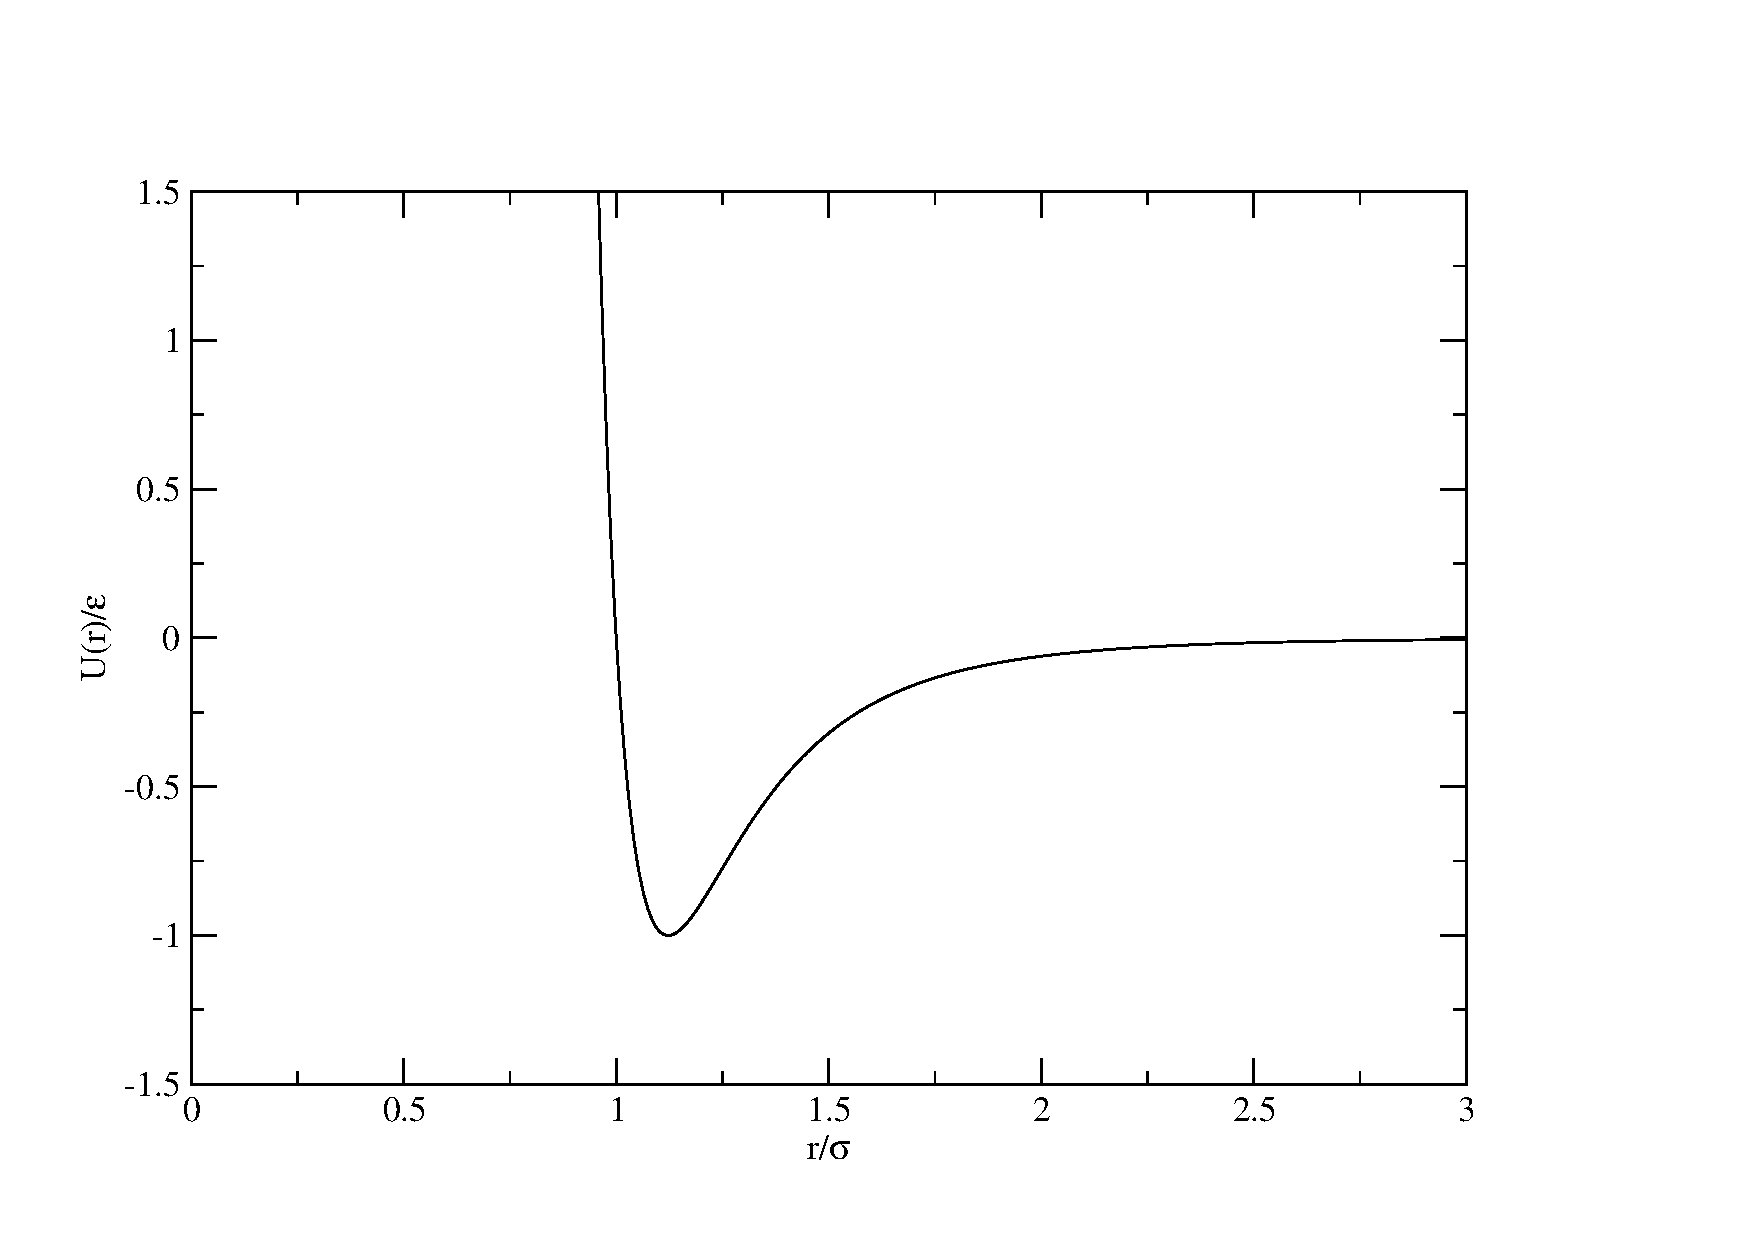
\includegraphics[clip,scale=0.45]{figures/ljPlot} 
    \caption[Lennard-Jones potential]{\label{fig:ljPot} Plot of the Lennard-Jones potential.}
  \end{center}
\end{figure}

The power 12 term, $\left(\sigma/r\right)^{12}$, gives the potential a
repulsive core caused by Pauli repulsion of overlapping electron
shells.  This repulsion is more accurately represented by an
exponential function which forms the basis of the Buckingham potential
\cite{Buckingham1938}.  However the Buckingham potential is not as
popular as the Lennard-Jones potential because the exponential
function is more computationally expensive to
calculate~\cite{White1997}.

The power 6 term, $\left(\sigma/r\right)^{6}$, in the Lennard-Jones
potential represents the attractive Van der Waals forces.  This
attractive well and repulsive core can be seen in the force plot 
of the Lennard-Jones potential, Fig.~\ref{fig:ljForce}.

\begin{figure}[htp] 
  \begin{center}
    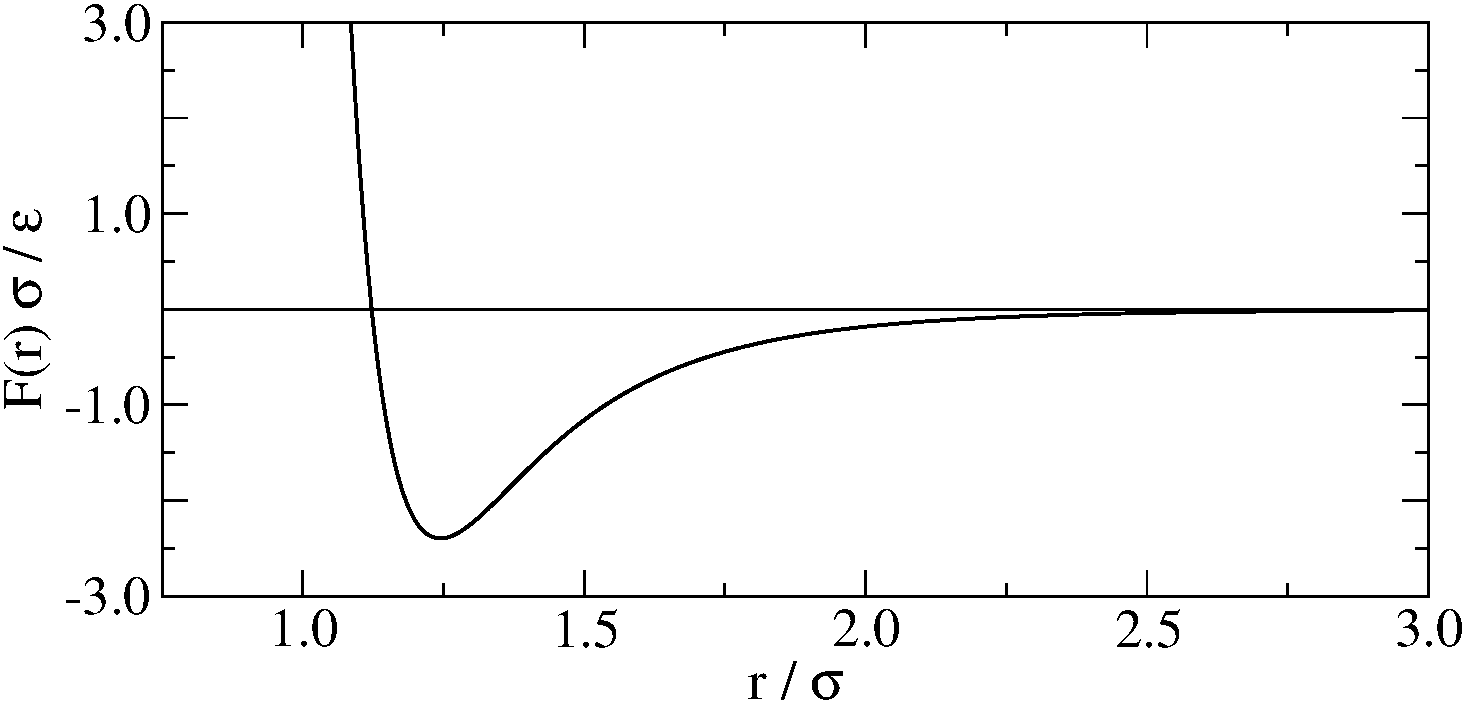
\includegraphics[clip,scale=0.45]{figures/ljForce} 
    \caption[Lennard-Jones force]{\label{fig:ljForce} Plot of the
      force between a pair of Lennard-Jones particles separated by a
      distance $r$, negative values represent an attractive force,
      while positive values indicate a repulsive force.}
  \end{center}
\end{figure}

\nomenclature[A]{CHARMM}{Chemistry at HARvard Molecular Mechanics}
While the Lennard-Jones potential simulates interactions between
single atoms very well, more complex potentials are needed to describe
particle chains.  An example of this is the CHARMM (Chemistry at
HARvard Molecular Mechanics) potential
(Eq.~\eqref{eq:CHARMMPotential})~\cite{MacKerell1998}.  
\begin{align}
  \label{eq:CHARMMPotential}
  \Phi &= \sum_{\text{bonds}}k_b(r-r_0)^2  
  + \sum_{UB}K_{UB}(S-S_0)^2 
  + \sum_{\text{angles}}k_\theta(\theta - \theta_0)^2 \nonumber\\
  &+ \sum_{\text{dihedrals}} k_\chi[1+\cos(n\chi - \delta)] 
  + \sum_{\text{improper}} k_\psi(\psi - \psi_0)^2 \nonumber\\
  &+ \sum_{i=1}^{N-1}\sum_{j>i}^{N}\left\{ 4 \varepsilon 
    \left[ \left( \frac{\sigma}{r_{ij}} \right)^{12}
      -\left( \frac{\sigma}{r_{ij}} \right)^{6} \right] 
    + \frac{q_iq_j}{r_{ij}}\right\}
\end{align}
Even in this more sophisticated potential, the Lennard-Jones potential
is being used to represent Van der Waals forces while Coulomb's Law
$\left(\frac{q_iq_j}{r_{ij}}\right)$ is modelling longer range
electrostatic interactions.  The first five terms of
Eq.~\eqref{eq:CHARMMPotential} are constraints on bond movements
(stretching, Urey-Bradley bond vibration, angle bending, dihedral
angle, and improper dihedral angle motion respectively, see
Ref.~\cite{Spoel2010} for descriptions of these bond movements).


\section{Discrete Potentials}

\begin{figure}[htp] 
  \begin{center}
    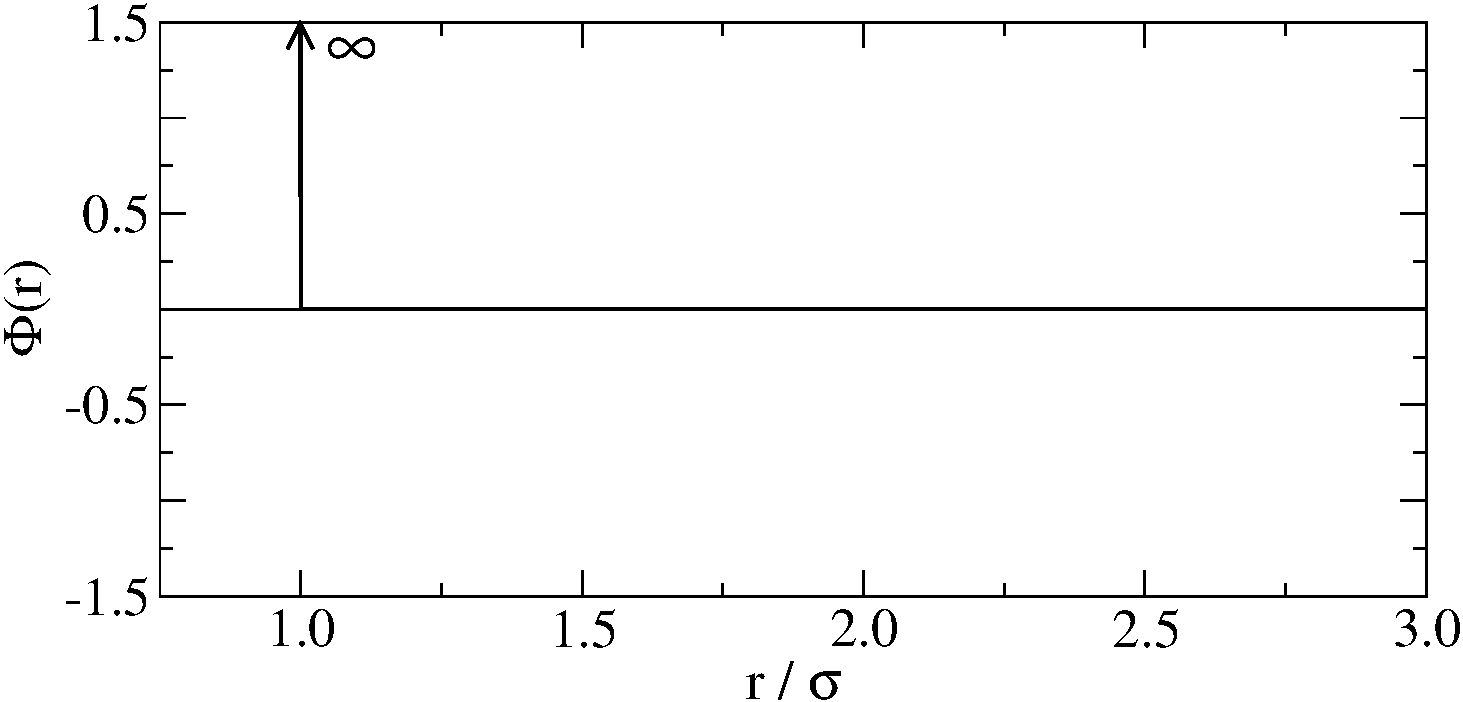
\includegraphics[clip,scale=0.45]{figures/hardsphere} 
    \caption[Hard sphere potential]{\label{fig:hardSphere} Plot of the
      hard sphere potential.}
  \end{center}
\end{figure}

Discrete potentials differ from continuous potentials because they
have discontinuities.  The simplest discrete potential is that of the
hard sphere (see Fig.~\ref{fig:hardSphere}). Hard spheres were the
first molecular models ever simulated~\cite{Alder1957} due to their
relative simplicity and are so-named as they cannot penetrate each
other due to the infinite overlap energy. The potential for hard
spheres is shown in Eq.~\eqref{eq:potentialHS}, where $\sigma$ is
the diameter of the spheres.
\begin{equation}
  \label{eq:potentialHS}
  \Phi(r) = 
  \begin{cases}
    \infty &\text{if }\; r < \sigma \\
    0 &\text{if }\; r \geq \sigma
  \end{cases}
\end{equation}

By calculating the force between two hard spheres using
Eq.~\eqref{eq:forcePotential} shows that hard spheres exert no force
until the particles collide whereupon they experience an infinite
repulsive force.  This means that hard spheres cannot overlap as they
would have to exceed an infinite force to do so.

The hard sphere potential can be elaborated upon by adding an
attractive well outside the hard core (see Fig.~\ref{fig:squareWell}).
This square well potential takes the form of
Eq.~\eqref{eq:potentialSW}~\cite{Barker1967}, where $\lambda$ is the
outer radius of the core in terms of the hard core diameter $\sigma$.
It should be noted here that at $r=\lambda\sigma$ the particle can
have a potential energy of either zero or $-\varepsilon$.

\begin{figure}[htp] 
  \begin{center}
    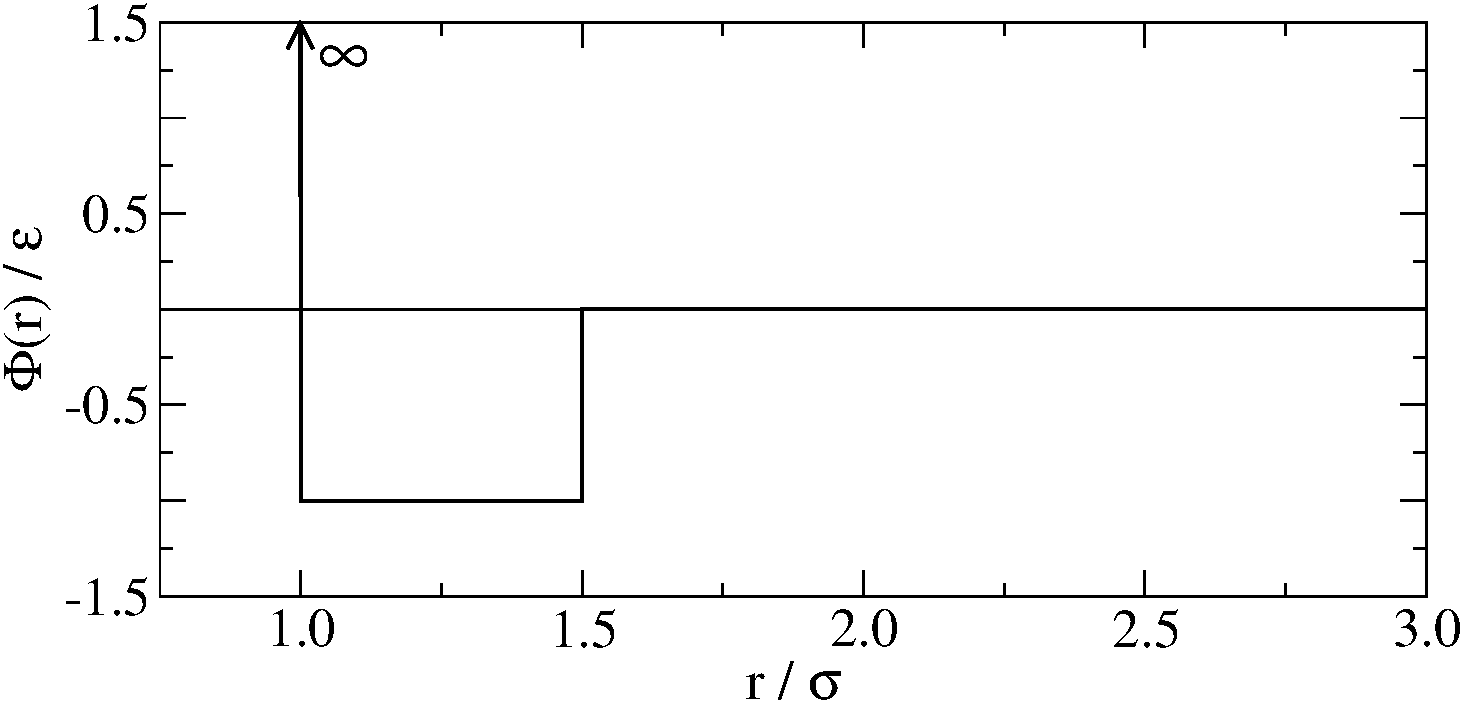
\includegraphics[clip,scale = 0.45]{figures/squareWell} 
    \caption[Plot of the square well potential]
    {\label{fig:squareWell} Plot of the square well potential with $\lambda=1.5$}
  \end{center}
\end{figure}

\begin{equation}
  \label{eq:potentialSW}
  \Phi(r) = 
  \begin{cases}
    \infty &\text{if }\; r < \sigma \\
    -\varepsilon &\text{if }\; \sigma \leq r \leq \lambda \sigma \\
    0 &\text{if }\; r \geq \sigma
  \end{cases}
\end{equation}

Stepped potentials are a combination of square wells and square
shoulders to mimic the behaviour of a continuous potential.  Many
types of stepped potentials have been developed in the literature.
Chapela \textit{et al.}~\cite{Chapela1989} created a stepped version
of the Lennard-Jones potential shown in Fig.~\ref{fig:chapelasteps}.

\begin{figure}[htp] 
  \begin{center}
    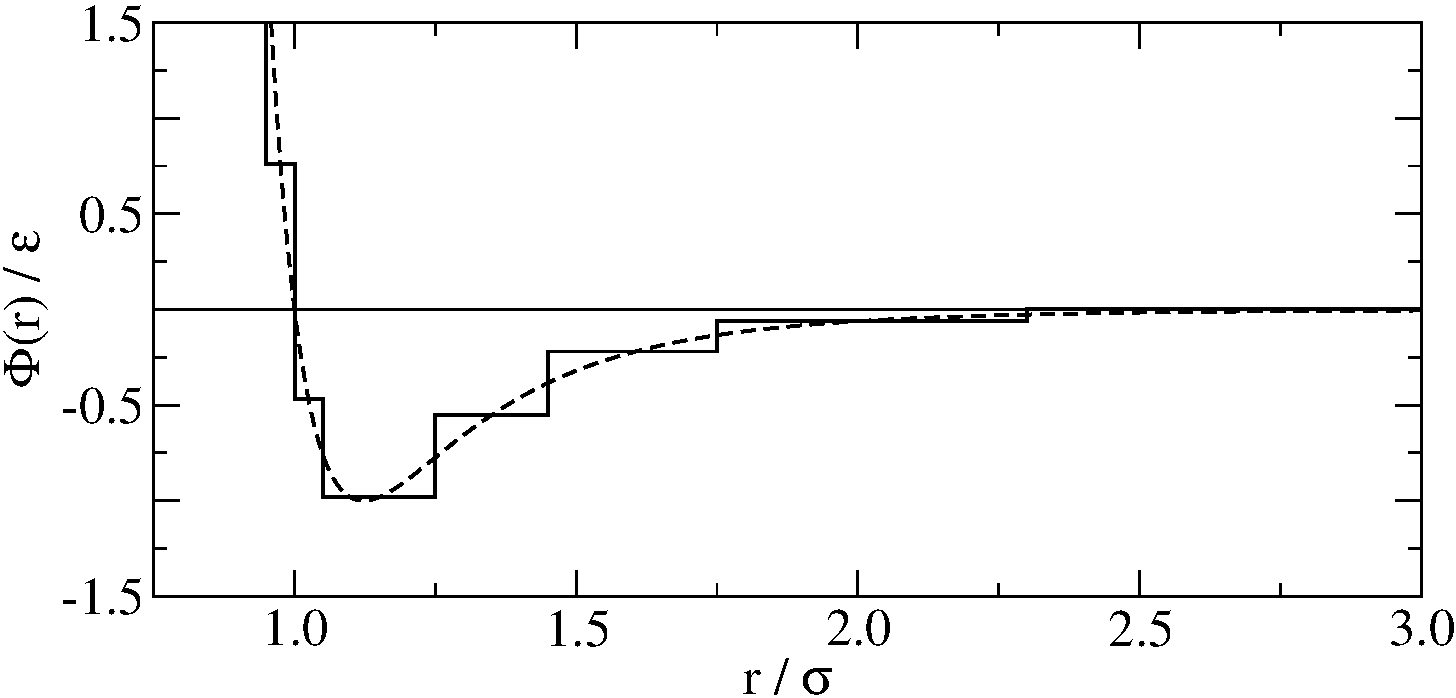
\includegraphics[clip,scale = 0.45]{figures/Chapela_Steps} 
    \caption[Plot of steps create by Chapela \textit{et al.}]
    {\label{fig:chapelasteps} A stepped version (solid line) of the
      continuous Lennard-Jones potential (dashed line) created by Chapela
      \textit{et al.}}
  \end{center}
\end{figure}

The SPEADMD (Step Potentials for Equilibria And Discontinuous
Molecular Dynamics)\nomenclature[A]{SPEADMD}{Step Potentials for
  Equilbria And Discontinuous Molecular Dynamics} project has created
stepped potentials (see Fig.~\ref{fig:SPEADMD}) that represent a range
of hydrocarbons~\cite{ElliotJr2002, Unlu2004, Vahid2010}.  These
potentials have been converted to equations of state using TPT that
match experimental values relatively well.

\begin{figure}[htp] 
  \begin{center}
    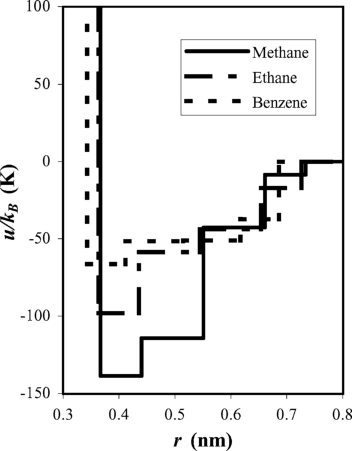
\includegraphics[clip,scale = 1.2]{figures/SPEADMD} 
    \caption [SPEADMD stepped potentials for methane, ethane and benzene]
    {\label{fig:SPEADMD} SPEADMD stepped potentials for methane,
      ethane and benzene~\cite{ElliotJr2002}.}
  \end{center}
\end{figure}

There are many validated continuous models in the literature, and
these potentials are very advanced.  Discrete potentials, on the other
hand, are still underdeveloped and underused. In the next chapter the
methods used to simulate these potential models will be described.
% Hard sphere,
%
%square well -> compare to LJ
%
%SPEAMD, PRIME
%
%Lead out with the two methods used to simulate these potentials are quite different....
\printbibliography[heading=thesisChapterBib] 


\chapter{Molecular Dynamics}

In this chapter the principles of molecular dynamics simulations are
discussed. First, the techniques used to solve Newton's Second Law of
Motion for both continuous and discrete potentials are described.
This is followed by a discussion of other important aspects of the
molecular simulation programs used in this dissertation.

\section{Applying Classical Mechanics to Molecular Systems}
%OR SOMETHING SIMILAR
%% Start with F=MA again, talk about how to solve it.

The most fundamental part of molecular dynamics is solving Newton's
Second Law of Motion (Eq.~\eqref{eq:Fmrddot}) for every particle in
the system.
\begin{equation} 
  \mathbf{F}_i = m_i \mathbf{a}_i = m_i \frac{\partial^2 \mathbf{r}_i}{\partial t^2}
  \label{eq:Fmrddot} 
\end{equation}
\nomenclature[V]{$\mathbf{r}_i$}{Position vector of particle $i$}
\nomenclature[V]{$t$}{Time} 
In Eq.~\eqref{eq:Fmrddot}, $\mathbf{r}_i$
is the position vector of particle $i$, and $t$ is time.  While the
forces acting on the particles can be calculated from their
intermolecular potentials, the future positions of the particles
become the solution of a set of simultaneous differential equations
(there are $3N$ differential equations to solve).  The techniques used
to solve these differential equations are different depending on
whether the potential is continuous or discontinuous.

\section{Force-Driven Simulation}
\subsection{Introduction}
For continuous potentials, it is not possible to solve
Eq.~\eqref{eq:Fmrddot} analytically for the future position of more
than two particles~\cite{Poschel2005}.  Therefore numerical methods
for solving differential equations have to be used; these are known as
numerical integrators.

\subsection{Integrators}
\label{sec:Integrator} 
Numerical integrators can be explained using a Taylor series:
\begin{equation} 
\mathbf{r}(t+\Delta t) = \mathbf{r}(t) + 
\frac{\partial\mathbf{r}(t)}{\partial t}(\Delta t) + 
\frac{1}{2}\frac{\partial^2\mathbf{r}(t)}{\partial t^2}\Delta t^2 + 
\frac{1}{3!}\frac{\partial^3\mathbf{r}(t)}{\partial t^3}\Delta t^3 
+ \frac{1}{4!}\frac{\partial^4\mathbf{r}(t)}{\partial t^4}\Delta t^4 
+ \mathcal{O}(\Delta t^5) \label{eq:Taylor} 
\end{equation}
\nomenclature[V]{$\Delta t$}{Simulator time increment}
where $\Delta t$ is the time-step and $\mathcal{O}(\Delta t^5)$
represents the higher order terms.

Although the Taylor series is exact, it is an infinite series which
makes it impractical to use. It must be truncated at some order. The
simplest integrator is Euler's Method:
\begin{subequations} 
  \label{eq:Euler}
  \begin{align}
    \mathbf{r}(t+\Delta t) &= \mathbf{r}(t) + \Delta t \mathbf{v}(t)
    +\mathcal{O}(\Delta t^2) \\
    \mathbf{v}(t+\Delta t) &= \mathbf{v}(t) + \Delta t \mathbf{a}(t)
    +\mathcal{O}(\Delta t^2)
  \end{align}
\end{subequations}
\nomenclature[V]{$\mathbf{v}_i$}{Velocity vector of particle $i$}
where $\mathbf{v}$ is the velocity vector of the particle and
$\mathcal{O}()$ indicates the truncation error in the integrator.
However, this method suffers from large errors and is highly unstable
(i.e.\ it amplifies any errors)~\cite{Haile1997} and is therefore
rarely used. The Verlet Integrator~\cite{Verlet1967} improves upon
Euler's method by combining the forward time-step with a reverse
time-step (Eq.~\eqref{eq:Verletpos}). Thihs method is actually third
order as the third (and first) derivative are cancelled out during its
derivation. The Verlet integrator does not include an equation to
calculate the future velocity, as the forces are only a function of
position; however, it is often desired to know the velocities to calculate
physical properties so the central difference approximation is often
used (Eq.~\eqref{eq:VerletVel}).
\begin{subequations} 
  \begin{align} 
    \mathbf{r}(t + \Delta t) &= 2\mathbf{r}(t) - \mathbf{r}(t - \Delta t) 
    + \mathbf{a}(t)\Delta t^2 + \mathcal{O}(\Delta t^4)
    \label{eq:Verletpos} \\ 
    \mathbf{v}(t+\Delta t) &= \frac{\mathbf{r}(t+\Delta t) -
      \mathbf{r}(t-\Delta t)}{2\Delta t}
    \label{eq:VerletVel} 
  \end{align}
\end{subequations}

Integrators suffer from two key failings that cause a systematic gain
of energy known as ``energy drift''. Firstly, integrators are based on
infinite Taylor series which cannot be fully implemented and have to
be truncated after a certain number of terms; this introduces
truncation error. Secondly, integrators are unable to predict values
of forces that have discontinuities in them, such as discrete
potentials or discontinuities introduced by truncating potentials to
improve simulator speed.  There are a couple of types of integrators
that try and reduce these problems.

The first method to improve the traditional integrator is the
predictor-corrector integrator. These use a truncated Taylor series to
calculate a predicted value for the future position and higher order
time derivatives. The force is calculated at this predicted position,
then the difference between the predicted acceleration, and the
corrected acceleration calculated from the force, is used to correct
the position and time derivatives.

The most common predictor-corrector integrator is that of Gear
\cite{Gear1971} using the 5th order algorithm. The predicted value for
the $n^{th}$ time derivative is shown in
Eq.~\eqref{eq:GearPredictor}. By defining $\Delta \mathbf{a} =
\mathbf{a}\,^{C} - \mathbf{a}\,^{P}$, where the superscripts $C$ and
$P$ denote the corrected and predicted values respectively, the
corrected time derivatives can be calculated using
Eq.~\eqref{eq:GearCorrector} with coefficients from
Eq.~\eqref{eq:GearCoeff}.
\begin{equation}
  \frac{\partial^{n}}{\partial t^{n}} \mathbf{r}\:^{P}(t+\Delta t)
  =\sum^{5}_{k=i} \frac{1}{k!}\frac{\partial^{n} }{\partial t^{n}}
  \mathbf{r}(t) \Delta t^{k} + \mathcal{O}(\Delta t^6)
  \label{eq:GearPredictor} 
\end{equation}
\begin{equation}
  \frac{\partial^{n}}{\partial t^{n}} \mathbf{r}\:^{C}(t+\Delta t)
  =\frac{\partial^{n} }{\partial t^{n}} \mathbf{r}\:^{P}(t+\Delta t)
  +\frac{c_i}{\Delta t^i} \left(\frac{\Delta t^2}{2}\Delta \mathbf{a}\right)
  \label{eq:GearCorrector} \end{equation} 
\begin{equation} 
  XOc_0 =
  \frac{3}{16},\;\;c_1 = \frac{251}{360},\;\; c_2 = 1,\;\; c_3 =
  \frac{11}{18},\;\; c_4 =
  \frac{1}{6},\;\; c_5 = \frac{1}{60} \label{eq:GearCoeff} 
\end{equation}\nomenclature[V]{$c_n$}{$n^{th}$ Gear coefficient}
Gear's algorithm, while more accurate at short time-steps than Verlet's
integrator~\cite{Haile1997}, loses precision at long time-steps and is
computationally expensive.  

The loss of precision at long time-steps is due to energy drift, a
failing all the integrators mentioned so far suffer from.  This is
reduced in another type of integrator: the symplectic integrator.
These have the useful property in that they, on average, conserve
energy~\cite{Hairer2003}. The most common symplectic integrator used
in MD is the Velocity Verlet Integrator~\cite{Swope1982} shown in
Eq.~\eqref{eq:VVerlet}.
\begin{subequations}
\label{eq:VVerlet}
\begin{align}
 \mathbf{r}(t + \Delta t) &= \mathbf{r}(t) + \mathbf{v}(t) \Delta t 
 + \frac{1}{2}\mathbf{a}(t) \Delta t^2 + \mathcal{O}(\Delta t^4)
 \label{eq:VVerletpos} \\
 \mathbf{v}(t+\Delta t) &= \mathbf{v}(t) + \frac{\mathbf{a}(t) 
   + \mathbf{a}(t+\Delta t)}{2}\Delta t
 \label{eq:VVerletVel}
\end{align}
\end{subequations}
The popularity of the Velocity Verlet is due to its computational
simplicity, accuracy and stability at relatively long
time-steps. It can even be expanded~\cite{Khakimov2002} to maintain its
accuracy and stability at very long time-steps at a small extra
computational cost. However the Velocity Verlet cannot be used in
systems that do not conserve energy, i.e.\ systems with dissipative
forces.

The Velocity Verlet integrator was chosen as the integrator
implemented in the force-driven simulation used in this dissertation.
The complexity and high computational cost of Gear's algorithm does
not compensate for any slight increase in accuracy over the Velocity
Verlet integrator.  Also since all the forces considered in this
dissertation are conservative, the use of a symplectic integrator over
non-symplectic integrators such as Gear's algorithm or the Verlet
integrator is sensible.

\subsection{General Algorithm}
The general algorithm for a force-driven simulator has not changed
since they were first introduced by Rahman~\cite{Rahman1964} who
predicted physical properties of liquid argon using a Lennard-Jones
potential.

Force-driven simulators move through time in uniform intervals of
time, $\Delta t$.  The particles' positions are calculated at the end
of each interval.  These new positions can then be used to calculate
the new forces acting on the particles. The overall algorithm for the
force-driven simulator written for this dissertation can be summarised
as follows:
\begin{enumerate} 
\item Initialisation.
\item Calculate particles' future positions using a numerical
  integrator (Velocity Verlet).
\item Calculate the forces acting on the particles from the
  intermolecular potential (Lennard-Jones).
\item Calculate the future velocities of particles .
\item Run thermostat.
\item Measure properties .
\item Repeat steps 2-6 for the desired number of iterations.
\end{enumerate} 

The techniques used to measure the physical properties of the system
will be discussed in Chap.~\ref{chap:Properties}.  The other parts
of the algorithm such as initialising the system and the thermostat
will be discussed in more depth later in this chapter, but first, the
solution of Newton's Equation of Motion for discontinuous potentials
is described.

\section{Event-driven Simulation}

\subsection{\label{sec:EDIntro}Introduction} 
The methods for integrating continuous potentials rely on calculating
the forces acting on the particles, however this is problematic when
working with discrete potentials.  The gradient (and hence the force) is
either infinite at the steps, or zero in between them.

Therefore a new technique for simulating these discrete potentials is
needed.  There is no force between the steps therefore the
acceleration is zero (Eq.~\eqref{eq:edfma}).
\begin{equation} 
  \mathbf{F}_i = m_i \mathbf{a}_i = 0 \label{eq:edfma}
\end{equation}
This can be integrated analytically to give:
\begin{equation}
  \mathbf{r}_i(t+\Delta t) = \mathbf{r}_i + \mathbf{v}_i\Delta t \label{eq:edNewPos}
\end{equation}
which allows the prediction of when particles reach a step, and using
the conservation of energy and momentum, the post collision velocities
of the particles can be calculated (this is expanded upon in
Sec.~\ref{sec:CollDyn}).  This method is known as event-driven
molecular dynamics and is an analytical solution of Newton's Second
Law of Motion.  This means that event-driven simulators do not suffer
from the numerical errors associated with the numerical integrators
described in Sec.~\ref{sec:Integrator}.

\subsection{Collision Time Prediction}
The prediction of the future positions of the particles using
Eq.~\eqref{eq:edNewPos} requires the time until the next
discontinuity is reached by any pair of particles. This section
outlines how these collision times are calculated.

For a hard sphere collision the distance between the particles must be
equal to the collision diameter of the particles:
\begin{equation}
 |\mathbf{r}_{ij} + \mathbf{v}_{ij}\Delta t| = \sigma \label{eq:edCollision}
\end{equation}
\nomenclature[V]{$\mathbf{r}_{ij}$}{Separation vector between particles $i$ and $j$}
\nomenclature[V]{$\mathbf{v}_{ij}$}{Relative velocity between particles $i$ and $j$}
where $\mathbf{r}_{ij} = \mathbf{r}_i - \mathbf{r}_j$ is the
separation vector between the two particles, while $\mathbf{v}_{ij} =
\mathbf{v}_i - \mathbf{v}_j$ is the relative velocity of the
particles.  Equation \eqref{eq:edCollision} can be squared to give:
\begin{equation}
 (\mathbf{r}_{ij} + \mathbf{v}_{ij}\Delta t)^2 = \sigma^2 \label{eq:edCollisionSqr}
\end{equation}
This is a quadratic equation for $\Delta t$ and the solution is shown
in Eq.~\eqref{eq:collEnterTime}.  

\begin{equation}
\Delta t = \frac{(-\mathbf{v}_{ij}\cdot\mathbf{r}_{ij}) \pm 
  \sqrt{(\mathbf{v}_{ij}\cdot\mathbf{r}_{ij})^2 - v_{ij}^2(r_{ij}^2 - \sigma^2)}}
       {v_{ij}^2} \label{eq:collEnterTime}
\end{equation}

There are two conditions that must be satisfied in order for a
collision to occur.  Firstly, the particles must be moving towards
each other (i.e.\ Eq.~\eqref{eq:collConditions1} must be true) and
secondly, the roots of Eq.~\eqref{eq:collEnterTime} must be real,
therefore Eq.~\eqref{eq:collConditions2} must apply. Physically this
represents the condition that the particles must pass close enough to
each other to collide.  
\begin{subequations}
  \begin{align}
    \mathbf{v}_{ij}\cdot\mathbf{r}_{ij} < 0 \label{eq:collConditions1}\\
    (\mathbf{v}_{ij}\cdot\mathbf{r}_{ij})^2 
    - v_{ij}^2(r_{ij}^2 - \sigma^2) \geq 0 \label{eq:collConditions2}
  \end{align}
\end{subequations}
While there are two solutions to Eq.~\eqref{eq:collEnterTime}, only
the earliest collision (the negative sign on the square root) needs to
be considered.  The second root gives the time when the particles
would leave each other after they passed through one another, which
cannot happen for hard spheres.

Since $\mathbf{v}_{ij}\cdot\mathbf{r}_{ij}$ must be negative for the
collision, there is the possibility of catastrophic cancellation
\cite{Goldberg1991}, if $(\mathbf{v}_{ij}\cdot\mathbf{r}_{ij})^2 \gg
v_{ij}^2(r_{ij}^2 - \sigma^2)$. Therefore it is advisable to use the
alternate form of the quadratic equation given in
Eq.~\eqref{eq:collEnterTimeAlt}~\cite{Poschel2005}.

\begin{equation}
\Delta t = \frac{r_{ij}^2 - \sigma^2}{(-\mathbf{v}_{ij}\cdot\mathbf{r}_{ij})
  + \sqrt{(\mathbf{v}_{ij}\cdot\mathbf{r}_{ij})^2 
    - v_{ij}^2(r_{ij}^2 - \sigma^2)}}
\label{eq:collEnterTimeAlt}
\end{equation}

When considering stepped potentials many of the same principles apply,
except there are now two additional possible ``collisions''. The first, when two
particles enter a step is treated identically to hard spheres. The
other event, when the particles leave the step, is calculated using
the second, later root of the quadratic.  In order to prevent loss of
numerical precision, the leaving time should be calculated using
Eq.~\eqref{eq:collExitTime}.

\begin{equation}
  \label{eq:collExitTime}
\Delta t = \frac{(-\mathbf{v}_{ij}\cdot\mathbf{r}_{ij}) +
  \sqrt{(\mathbf{v}_{ij}\cdot\mathbf{r}_{ij})^2 - v_{ij}^2(r_{ij}^2 - \sigma^2)}}
     {v_{ij}^2}
\end{equation}
This allows the calculation of the time when a discontinuity occurs.
The next section will discuss the technique used to solve the
discontinuity itself.

\subsection{Collision Dynamics \label{sec:CollDyn}}
Once the time of the next collision is known, the particles can be
moved to their new locations, using Eq.~\eqref{eq:edNewPos}. However,
in order to predict future collisions the post-collision velocities of
the colliding particles must also be calculated.  

The simplest collision between two particles is an elastic bounce,
where the velocities and just exchanged along the separation vector
between the two particles~\cite{Haile1997}.  The change in velocity
during the collision for particles $i$ and $j$ is given by:
Eq.~\eqref{eq:postVBounce}.

\begin{subequations}
  \label{eq:postVBounce}
  \begin{align}
    \Delta\mathbf{v}_i &= -(\mathbf{v}_{ij}\cdot\mathbf{\hat{r}}_{ij})\mathbf{\hat{r}}_{ij} \\
    \Delta\mathbf{v}_j &= (\mathbf{v}_{ij}\cdot\mathbf{\hat{r}}_{ij})\mathbf{\hat{r}}_{ij}
  \end{align}
\end{subequations}
\nomenclature[V]{$\Delta \mathbf{v}_i$}{Change in the velocity of particle $i$ during a collision}
\nomenclature[S]{$\hat{x}$}{Unit vector}
For stepped potential system, the collision dynamics are more complex.
When two particles collide they must pay an energy ``cost'' to proceed
through the step.  This energy cost, $\Delta \Phi$, is the difference in
the energy of the current step and the step the particles are going
into, and is shown in Eq.~\eqref{eq:energyCost}.

\begin{equation}
  \label{eq:energyCost}
  \Delta \Phi = \Phi_{\text{next step}} - \Phi_{\text{current step}}
\end{equation}
\nomenclature[V]{$\Delta \Phi$}{Change in potential energy during
  a collision} 
If the kinetic energy of the particles is insufficient,
the pair bounce off the step and the post-collision velocities are
calculated using Eq.~\eqref{eq:postVBounce}. However, if the particles
have sufficient energy i.e.\ the inequality Eq.~\eqref{eq:kineticCost}
is true, then the particles can enter the step.

\begin{equation}
\label{eq:kineticCost}
  \frac{1}{4}m(\mathbf{v}_{ij}\cdot\mathbf{\hat{r}}_{ij})^2 > \Delta \Phi
\end{equation}

The change in the velocities of particles $i$ and $j$ after going
through a step are shown in Eq.~\eqref{eq:postVCapture} where $A$ is
given in Eq.~\eqref{eq:changeMomentum}; the derivation of these
equations is given in Appendix~\ref{app:derivation}.  If the particles
are entering a step, the positive square root of $A$ is used, whereas
if the particles are leaving a step it is the negative square root
that should be used.

\begin{subequations}
  \label{eq:postVCapture}
  \begin{align}
    \Delta\mathbf{v}_i &= \frac{A}{m} \mathbf{\hat{r}}_{ij} \\
    \Delta\mathbf{v}_j &= -\frac{A}{m}\mathbf{\hat{r}}_{ij}
 \end{align}
\end{subequations}
\begin{equation}
  A = -\frac{m}{2}\left((\mathbf{v}_{ij}\cdot\mathbf{\hat{r}}_{ij}) \pm
    \sqrt{(\mathbf{v}_{ij}\cdot\mathbf{\hat{r}}_{ij})^2 - \frac{4}{m}\Delta \Phi}\right)
  \label{eq:changeMomentum}
\end{equation}
\nomenclature[V]{$A$}{Momentum change during a collision}
It can be noticed that Eq.~\eqref{eq:postVBounce} can be derived from
Eqs.~\eqref{eq:postVCapture} and \eqref{eq:changeMomentum} by setting
$\Delta \Phi=0$.
\subsection{General Algorithm for Event-Driven Simulation}

The algorithm used for the event-driven simulation is very similar to
the algorithm used by Alder and Wainwright~\cite{Alder1959} and is
shown below:

\begin{enumerate} 
\item Initialisation.
\item Find the next event.
\item Process the event.
\item Update the event list.
\item Measure properties.
\item Repeat steps 2-5 for the desired number of events.
\end{enumerate} 

Several parts of this algorithm apply to both event and force-driven
simulations are discussed in more depth in the following sections.

\section{Initialisation \label{sec:initMD}} 
Both the force and even-driven simulators written for this
dissertation initialise the particles in the same way. The particles
are initially placed in a Face Centred Cubic (FCC)
\nomenclature[A]{FCC}{Face Centred Cubic} structure. The use of the
FCC lattice is common when simulating Lennard-Jones potentials as it
is the closest possible packing of mono-sized spheres.

The particle velocities are then assigned randomly from a Gaussian
distribution with a mean, $\mu = 0$, and a standard deviation, $\sigma
= \sqrt{T^{*}}$, where $T^{*}$ is the desired reduced temperature. The
velocities are then rescaled to ensure there is no net shift in linear
momentum in any direction by applying Eq.~\eqref{eq:zeroLinearP}.

\begin{equation} 
  \mathbf{v}_{i}^{\text{new}} = \mathbf{v}_{i}^{\text{old}} - \frac{1}{N}
  \sum^{N}_{i}\mathbf{v}_{i}^{\text{old}}
  \label{eq:zeroLinearP} 
\end{equation}

\section{Periodic Boundary Conditions}
When simulating a system it is necessary to have a boundary to prevent
the particles from moving away from each other into infinity.  However
solid walls have a large effect on the properties of a system so an
alternative method is needed.  Since the earliest MD simulations
\cite{Alder1959}, periodic boundary conditions have been used to solve
this problem.

\begin{figure}[htp] 
  \begin{center}
    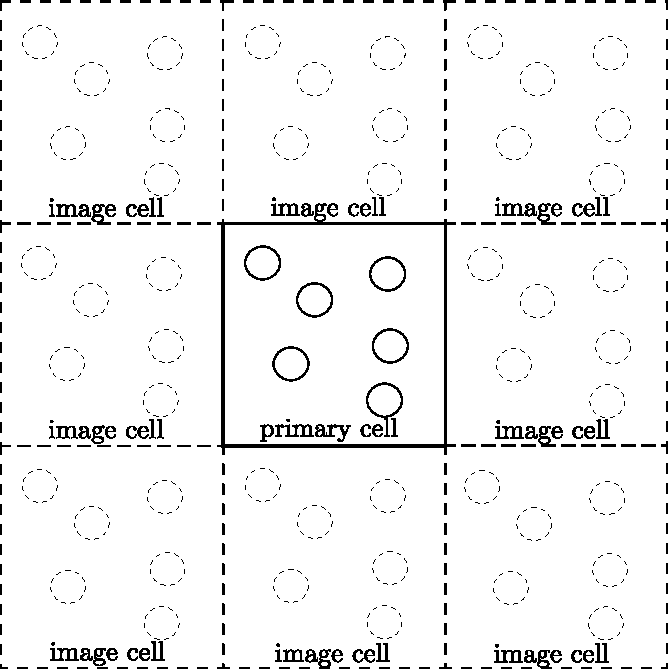
\includegraphics[clip, scale = 0.8]{figures/PBC} 
    \caption [Figure showing 2D periodic boundary conditions]
    {\label{fig:PBC} Figure showing 2D periodic boundary
      conditions. Only the nearest eight images (dashed) to the simulated
      system (solid) are shown.}
  \end{center}
\end{figure}

The concept behind periodic boundary conditions is to create a
pseudo-infinite system made up of tessellated images of the simulated
system (as shown in Fig.~\ref{fig:PBC}).  When a particle leaves the
primary cell, its image enters from the opposite side.  This ensures
mass is conserved in each cell.  

The problem with this is that particles can interact with multiple
images of another particle.  Molecular simulations use the minimum
image criterion to ensure particles only interact with the
closest image of another particle. In event-driven simulators only the
collision time with the nearest image is considered, but this is not
necessarily the same image as the one the particle will collide with
next.  The event-driven simulator in this dissertation recalculates the
collision time if the particle has travelled far enough ($1/4 (\text{box
length}-\sigma)$) to collide with an image other than the nearest one.

\section{Thermostat}

All simulations in this dissertation use the canonical NVT ensemble,
i.e.\ the number of particles, $N$, the volume of the system, $V$ and
the temperature, $T$ were kept constant during the simulation.  While
keeping the number of particles and system size constant is simple,
controlling the temperature is more complex.

The simplest method for controlling the temperature is to rescale the
particle velocities to match the desired temperature using
Eq.~\eqref{eq:tempRescale}.

\begin{equation}
  \label{eq:tempRescale}
  \mathbf{v}_{\text{new}} = \mathbf{v}_{\text{old}} \sqrt{\frac{T_{\text{desired}}}{T_{\text{current}}}}
\end{equation}
\nomenclature[V]{$T$}{Temperature of the system}
\nomenclature[V]{$V$}{Volume of the system}
However this does not allow energy fluctuations that should exist in a
NVT system, therefore an Andersen thermostat~\cite{Andersen1980} is
used.  An Andersen thermostat works by colliding a random particle
with a ghost particle at the desired temperature.  In this
force-driven simulation, this is achieved by reassigning the
velocities of ~5\% of particles from a Gaussian distribution at the
correct temperature (similar to Sec.~\ref{sec:initMD}) on every time-step.

For the event-driven simulation a more sophisticated implementation is
used.  An extra event is created for the thermostat, with the time to
the event calculated from an exponential distribution with a rate of
20 thermostat events per unit time.  The reason an exponential
distribution is used is that the thermostat is an example of a Poisson
Process, where an event happens at a constant rate yet each event
occurs independently.  At this thermostat event a random particle has
its velocities reassigned from the Gaussian distribution at the
desired temperature, similar to the force-driven simulation.

\section{Optimisation \label{sec:Optimisation}}
Due to the time-consuming nature of computer simulations there are a
number of techniques used to reduce their running times.  This section
will outline a number of the techniques implemented in the programs
coded for this dissertation.

\subsection{Truncation of the Potential}
Since the calculation of the forces on the particles is the most
time-consuming part of force-driven simulations~\cite{Frenkel2002},
almost all optimising techniques focus on this aspect.

A simple yet effect technique to improve simulation speed is to
truncate the potential.  Since continuous potentials tend to zero as
particles get further away from each other, significant time can be
saved by selecting a cut-off radius at which the potential is taken to
be zero.  The form of a truncated potential is shown in
Eq.~\eqref{eq:truncatePotential}.  For the Lennard-Jones potential a
cut-off radius of $3\sigma$ is used as $\Phi(3\sigma) =
-0.00548\varepsilon$ and $F(3\sigma) = -0.0109\varepsilon/\sigma$ are
both approximately 0.5\% of the minimum energy or maximum attractive
force respectively.

\begin{equation}
  \label{eq:truncatePotential}
  \Phi(r) = 
  \begin{cases}
    \Phi(r) &\text{if }\; r \leq r_{\text{cut-off}} \\
    0 & \text{if }\; r > r_{\text{cut-off}} 
  \end{cases}
\end{equation}

\subsection{Neighbour Lists}
While truncating the potential prevents the calculation of the forces
it still requires the computation of the distance between particles.
These extraneous calculations can be eliminated by using a neighbour list.

There are two main types of neighbour list used in molecular dynamics
simulations.  The first is the use of Verlet lists~\cite{Verlet1967},
and this is the type used in this dissertation for the force-driven
simulation.  A Verlet list is a list of all the particles within a
certain radius of a particle.  If this list was updated every
time-step, this would be no improvement on the original method, but by
making the Verlet radius larger than the truncation radius, this list
can be used for multiple time-steps.  Haile~\cite{Haile1997} recommends
using a Verlet radius of $3.3\sigma$, and updating the list every $10$
time-steps, and this is what was done in this dissertation for the
force-driven simulator.

Another method is to use cell-linked lists~\cite{Poschel2005}, which
involves dividing the system into a grid and only the particles in the
same cell or a neighbouring cell are taken into account.  This method
can be inefficient as the length of each cell must be at least
the truncation cut-off radius wide to prevent particles being missed
out.  This means a volume of $27r_{\text{cut-off}}^3$ (as in 3
dimensions each cell has 26 neighbours) are considered but only
particles within the spherical volume $\frac{4}{3}\pi
r_{\text{cut-off}}^3$ should be checked; this means the volume tested
is over six times larger than it needs to be.

Mattson and Rice~\cite{Mattson1999} improve this by reducing the
length of each cell to less than the cut-off radius, but this results
in more neighbouring cells having to be checked i.e. for a cell length
of $0.5r_{\text{cut-off}}$ the nearest 124 (a $5\times 5\times 5$
grid) cells are considered neighbours. This means there is a
compromise as smaller cells mean that less volume is checked, but also
means the cell lists are made obsolete quicker and therefore have to
generated more frequently.

Neighbour lists can be implemented in event-driven simulators as well,
and are of the cell-linked list type as this best utilises the
event-driven nature of these simulators.  However due to time
constraints one was not implemented in the event-driven simulator used
for this dissertation.

\subsection{Optimisation for Event-Driven Simulators}
Although no neighbour list was implemented in the event-driven simulator
a number of other optimisation techniques were used.  Due to the more
complex nature of event-driven simulations there are a larger number
of methods used to increase simulator efficiency.  Whereas in the
force-driven simulator the calculation of the forces was the most
time-consuming part, in event-driven simulators it is calculation of
the collision time that is the most computationally intensive.

When two particles collide, only the velocities of those two particles
change.  This means that the collision times for every collision that
did not involve either of the two particles is still valid.  Rather
than recalculating these collision times every cycle, they are stored
in an event list and are only updated when they change.  

The inclusion of an event list means it must be sorted to find the
earliest event. The time taken to sort the event list increases with
the number of events therefore it is desired to have as short a list
as possible (there are examples of $\mathcal{O}(1)$ priority queues
that do not have this problem~\cite{Paul2007}).  Therefore every
particle has its own event list and only the earliest event of each
particle is stored in the master event list.  The event list used in
this dissertation was not fully sorted, it was only searched for the
earliest event.

However when two particles collide their events with every other
particle become obsolete, but these events are spread over every
particles' individual event list.  The time spend searching for and
deleting these obsolete events can be saved by only updating them when
they reach the top of the event list.  A parameter such as the number
of collisions the particles have undergone is used to decide whether
an event is valid and can be executed or obsolete and needs to be
updated~\cite{Poschel2005}.

These optimisation techniques can increase the speed of a simulation
by an order of magnitude or more and allow larger systems of particles
to be simulated for longer periods of time which ensures accuracy of
the results obtained in this dissertation.

\section{Summary}

The outlines for the algorithms for event-driven and force-driven
simulators have been given in this chapter.  Force-driven simulators
are much more popular due to their simplicity but their solution is
only approximate and is subject to large numerical errors.

Event-driven simulators do not have these same errors but they are
significantly more complex.  This is highlighted in that over 2200
lines of code are required for the event-driven simulator whereas the
force-driven simulator needs less than 1000 to simulate the same
system.

While event-driven simulators are more accurate, and hence more
desirable, all the sophisticated potentials in the literature are
continuous.  This means that force-driven simulators must be used to
simulate these models.  The aim of this dissertation is to bridge the
gap between these two classes of potentials and this will be discussed
in Chap.~\ref{chap:cont2dis}. In the following chapter the methods
used to measure some of the properties of molecular systems so the
results from continuous and discontinuous models can be compared.

\printbibliography[heading=thesisChapterBib] 

\chapter{Measuring Thermodynamic Properties}
\label{chap:Properties}
Until now only the motion of the system has been calculated, but the
positions and velocities are only the means to an end.  The real
purpose of a molecular dynamics simulation is to the measure
thermodynamic properties of the system.  First, the need for time
averaging of these properties is discussed, and this is followed by a
description of the techniques used to measure various properties
(energy, temperature, pressure, radial distribution function). 
Finally, the system of units commonly used in molecular dynamics, and
the system used in this dissertation is discussed.

\section{Time Averaging}
Molecular dynamics is a useful tool to predict macroscopic properties
of molecular systems. However, even when the system is at equilibrium,
the values of these properties fluctuate around a mean (see
Fig.~\ref{fig:fluctuations}) therefore it is common to take time
averages of these values. These time averages are denoted with angle
brackets $\langle\:\: \rangle$, and the time average of a property,
$A$, is shown in Eq.~\eqref{eq:TAdef}~\cite{Haile1997}.
\nomenclature[S]{$\langle\:\: \rangle$}{Time average}
\begin{figure}[htp] 
  \begin{flushleft}
    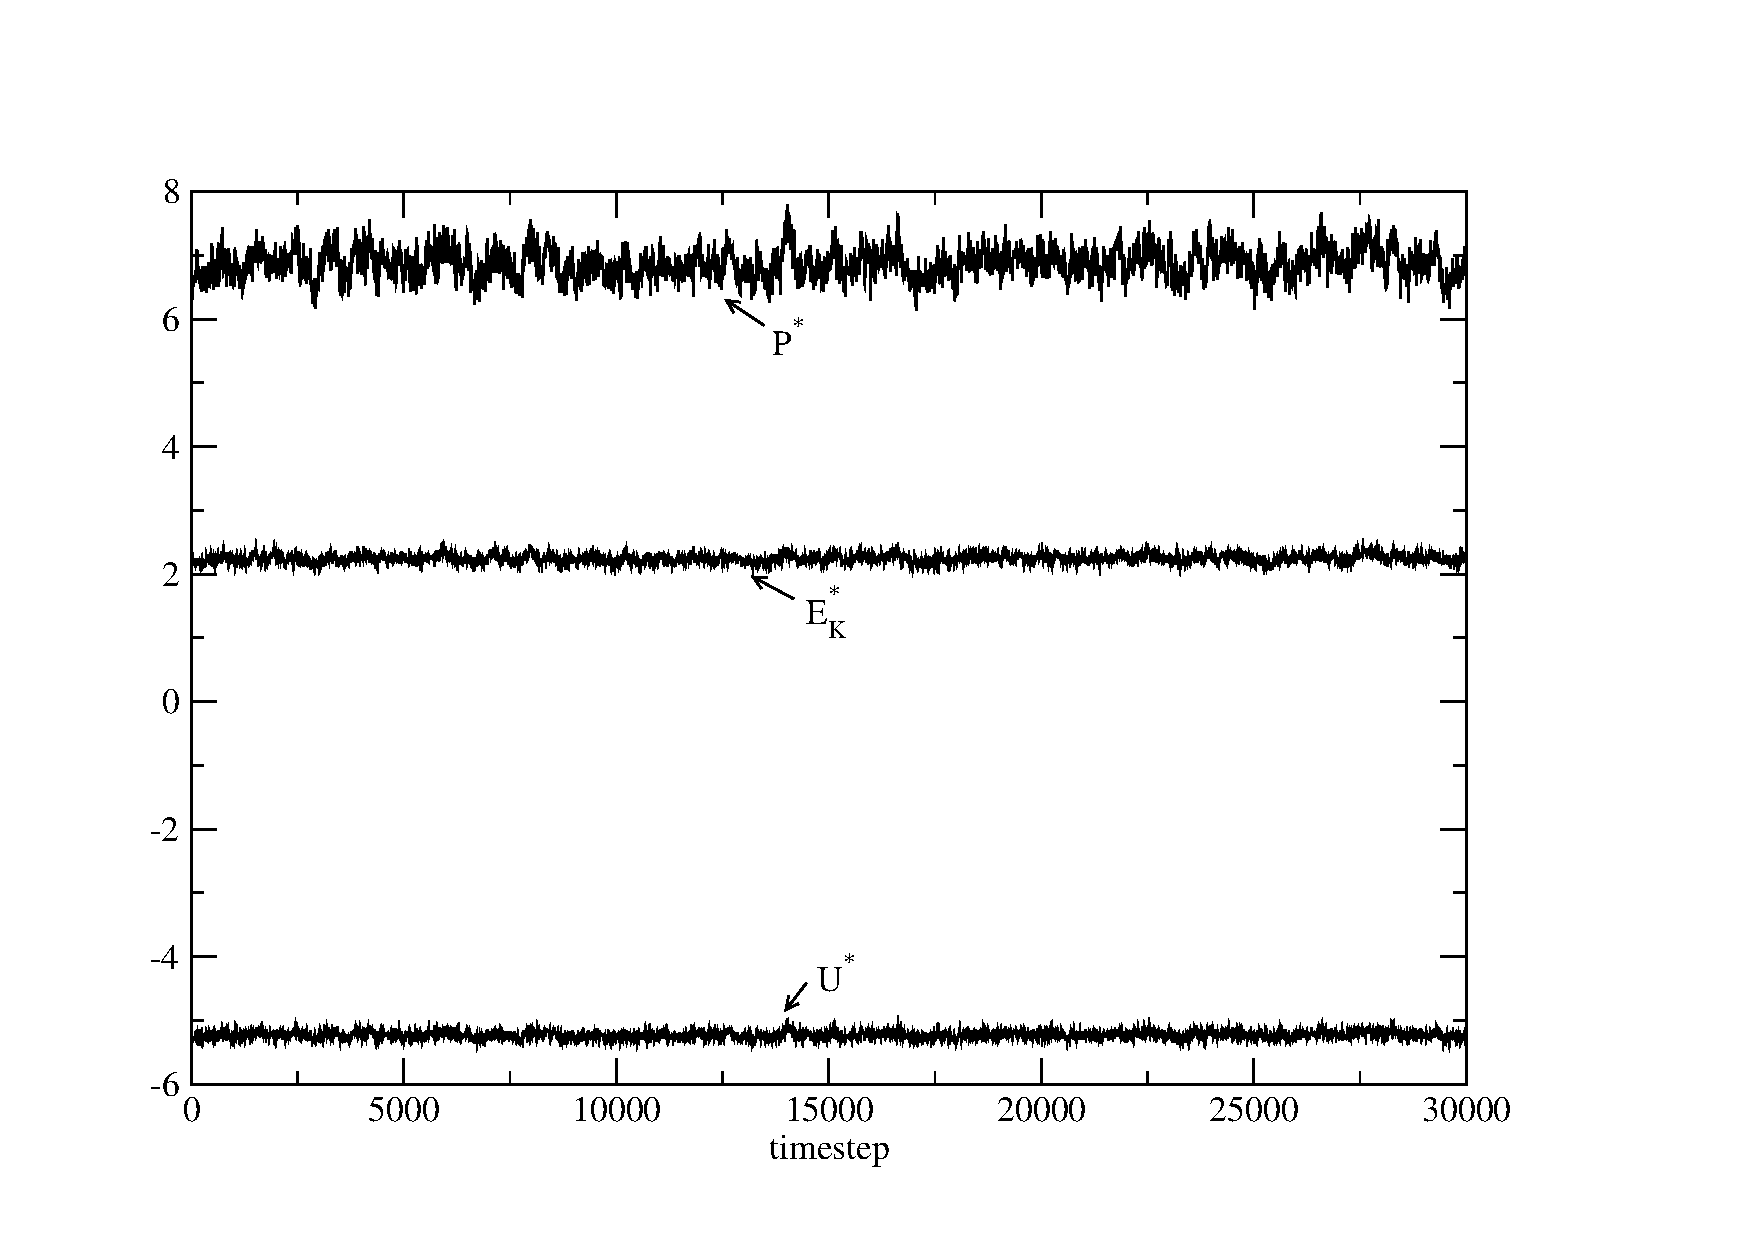
\includegraphics[clip,scale = 0.55]{figures/energyplot} 
    \end{flushleft}
    \caption[Fluctuation of system properties]
    {\label{fig:fluctuations} Plot showing fluctuation of pressure
      ($P^*=P\sigma^3/\varepsilon$), kinetic energy per particle
      ($E_K^*=E_K/N\varepsilon$) and potential energy per particle
      ($\Phi^*=U/N\varepsilon$).  Results are from a force-driven
      simulation involving 864 particles, at a density $\rho^*=0.9$
      and temperature $\langle T^*\rangle=1.497$. Values were
      collected every 10 time-steps where each time-step was $\Delta t^*
      = 0.005$.}
\end{figure}

\begin{equation}
  \label{eq:TAdef}
  \langle A \rangle = \lim_{t \to \infty} \frac{1}{t}  \int^{t_0+t}_{t_0}A(\tau) {\rm d}\tau
\end{equation}
\nomenclature[V]{$\tau$}{Dummy time variable in time average integrals}
This time average can be calculated precisely in event-driven
simulations for several properties such as pressure, kinetic energy
and potential energy.  These only change at collisions and therefore
are constant for the time between the collision and can be calculated
using:
\begin{equation}
  \label{eq:TASum}
  \langle A \rangle = \frac{1}{t}\sum^{N_{\text{coll}}}A(t_c)\Delta t
\end{equation}
\nomenclature[V]{$t_c$}{Time between collisions}
where $N_{\text{coll}}$ is the number of collisions in time, $t$, and
$\Delta t$ is the time between the collision at time $t_c$ and the
next collision.

In force-driven simulators all properties change continuously and
hence time averages cannot be calculated precisely, however
approximations can be made. If properties are measured every uniform
period of time, the time average can be approximated by:
\begin{equation}
  \label{eq:TAforcedriven}
  \langle A \rangle = \frac{1}{M} \sum^{M}_{1}A(\tau)
\end{equation}
where $M$ is the number of measurements taken.
\nomenclature[V]{$M$}{Number of measurements taken}
\section{Energy \label{sec:Energy}}
Perhaps one of the most important properties to measure in MD
simulations is the total internal energy of the system.  For isolated
systems, i.e.\ systems where mass or energy cannot enter or leave the
system, this internal energy is the sum of kinetic and potential
energy (Eq.~\eqref{eq:internalE}).

\begin{equation}
  U = E_K + \Phi \label{eq:internalE}
\end{equation}
\nomenclature[V]{$U$}{Total internal energy of the system}
The total kinetic energy in the system is the sum of the kinetic
energy of each particle, as shown in Eq.~\eqref{eq:totalEK}.

\begin{equation}
  \label{eq:totalEK}
  E_K = \sum_i^N mv_i^2
\end{equation}
\nomenclature[V]{$E_K$}{Kinetic energy of the system}
The potential energy of the system is the sum of the potential energy
between every pair of particles (for a pairwise potential), and is
shown in Eq.~\eqref{eq:totalU}.

\begin{equation}
  \label{eq:totalU}
  \Phi = \underset{i\;\;<\;\;j}{\sum\sum}\Phi(r_{ij})
\end{equation}
\nomenclature[V]{$\Phi$}{Potential Energy of the system}
Event-driven simulators strictly conserve energy, therefore the
kinetic and potential energy can be measured at the beginning of the
simulation and then updated whenever either changes e.g.\ when a
collision occurs.

\section{Temperature}

The velocity distribution of particles is given by the Maxwell
distribution~\cite{Haile1997}:
\begin{equation}
  \label{eq:MaxwellDist}
  f(v_x)dv_x = \sqrt{\frac{m}{2\pi k_BT}}e^{-\frac{mv_x^2}{2k_BT}} 
\end{equation}
where $k_B$ is the Boltzmann Constant.
\nomenclature[V]{$k_B$}{Boltzmann Constant}
\nomenclature[F]{$f(v_x)$}{Probability distribution of equilibrium velocities}
This is the form of a Gaussian distribution and it can be shown
\cite{Landau1968} that the mean square velocity in any direction is as
shown in Eq.~\eqref{eq:MSV}.

\begin{equation}
  \label{eq:MSV}
  \bar{v}_x^2 = \frac{k_BT}{m}
\end{equation}
\nomenclature[S]{$\bar{x}$}{Mean value}
Making the assumption that the velocity distribution is the same in
each direction (which is valid if the system is in equilibrium), the
temperature can be expressed as Eq.~\eqref{eq:Temperature}, by taking
the average temperature in each direction.

\begin{equation}
\label{eq:Temperature}
  T^* = k_BT = \frac{mv^2}{3N} = \frac{2}{3N}E_K
\end{equation}
This allows the calculation of the temperature from the kinetic energy
of the system.
\section{Pressure \label{sec:Pressure}}

The pressure in a molecular dynamics simulation is calculated using
the virial equation of state (Eq.~\eqref{eq:virialEOS})
\cite{Landau1968}.

\begin{equation}
  \label{eq:virialEOS}
  \frac{PV}{Nk_BT} = 1 + B_2\rho + B_3\rho^2 + B_4\rho^3 + ...
\end{equation}
\nomenclature[V]{$P$}{Pressure of the system}
\nomenclature[V]{$\rho$}{Density of the system}
\nomenclature[V]{$B_n$}{$n^{th}$ Virial coefficient}
The coefficients, $B_2, B_3, B_4, ...$ are known as the second, third,
fourth, etc. virial coefficients.  Values for these virial
coefficients are available in the literature for common potentials
such as hard spheres~\cite{Labik2005} or
Lennard-Jones~\cite{Schultz2009}. Physically these coefficients
represent the contribution to the pressure from the interaction of a
particle with two, three, four, etc. other particles.

The second virial can be calculated using
Eq.~\eqref{eq:secondVirial}~\cite{Smith2005} in three
dimensions. Similar expressions can be written for the higher virial
coefficients however the solution to these is very time-consuming.
\begin{equation}
  \label{eq:secondVirial}
  B_2 = -2\pi \int^\infty_0 \left(e^{\Phi(r)/k_BT}-1\right)r^2{\rm d}r
\end{equation}
Therefore an alternative expression to measure the contribution to the
pressure of all the virial coefficients has been created for both
simulation methods by using kinetic theory and measuring momentum flux
during the simulation.  In force-driven simulations, the second virial
can be calculated using Eq.~\eqref{eq:virialMD}~\cite{Haile1997}.

\begin{equation}
  \label{eq:virialMD}
  \frac{PV}{Nk_BT} = 1 +
  \frac{1}{3NkT}\left \langle\underset{i\;\;<\;\;j}{\sum\sum}\mathbf{F}_{ij}\cdot\mathbf{r}_{ij} \right\rangle
\end{equation}

Calculating the pressure in event-driven simulators is more complex
due to the lack of forces in the simulation, however by keeping track
of the momentum flux at each collision an average pressure can be
calculated using Eq.~\eqref{eq:virialED}~\cite{Lue2005}.  Here
$N_{\text{coll}}$ is the total number of collisions during the time
$t$.

\begin{equation}
  \label{eq:virialED}
  \frac{PV}{Nk_BT} = 1 +
  \frac{m}{3}\frac{N_{\text{coll}}}{Nt}\langle\mathbf{r}_{ij}\cdot\Delta \mathbf{v}_i\rangle_{\text{coll}}
\end{equation}
\section{Radial Distribution Function}
\label{sec:RDF}
One of the most important measurements in molecular dynamics is the
radial distribution function (RDF)\nomenclature[A]{RDF}{Radial
  Distribution Function}.  The RDF provides information concerning the
arrangement of the particles, and can be determined
experimentally~\cite{Yarnell1973}.  This means that the RDF can be
used to determine the agreement of MD simulations and experimental
results.

Statistically, the RDF is the ratio of the probability of finding a
particle a distance $r$ from another particle to the expected
probability if the particles were randomly distributed
~\cite{Allen1987}. Since potentials usually have a hard core there is
very little chance of finding a particle within the radius of another
particle, therefore the RDF is zero very close to the particle.
However, as the radial distance tends to infinity the probability of
finding a particle tends to the randomly distributed probability so
the RDF tends to one, which can be seen in Fig.~\ref{fig:rdfsmooth}.

\begin{figure}[htp] 
  \begin{center}
    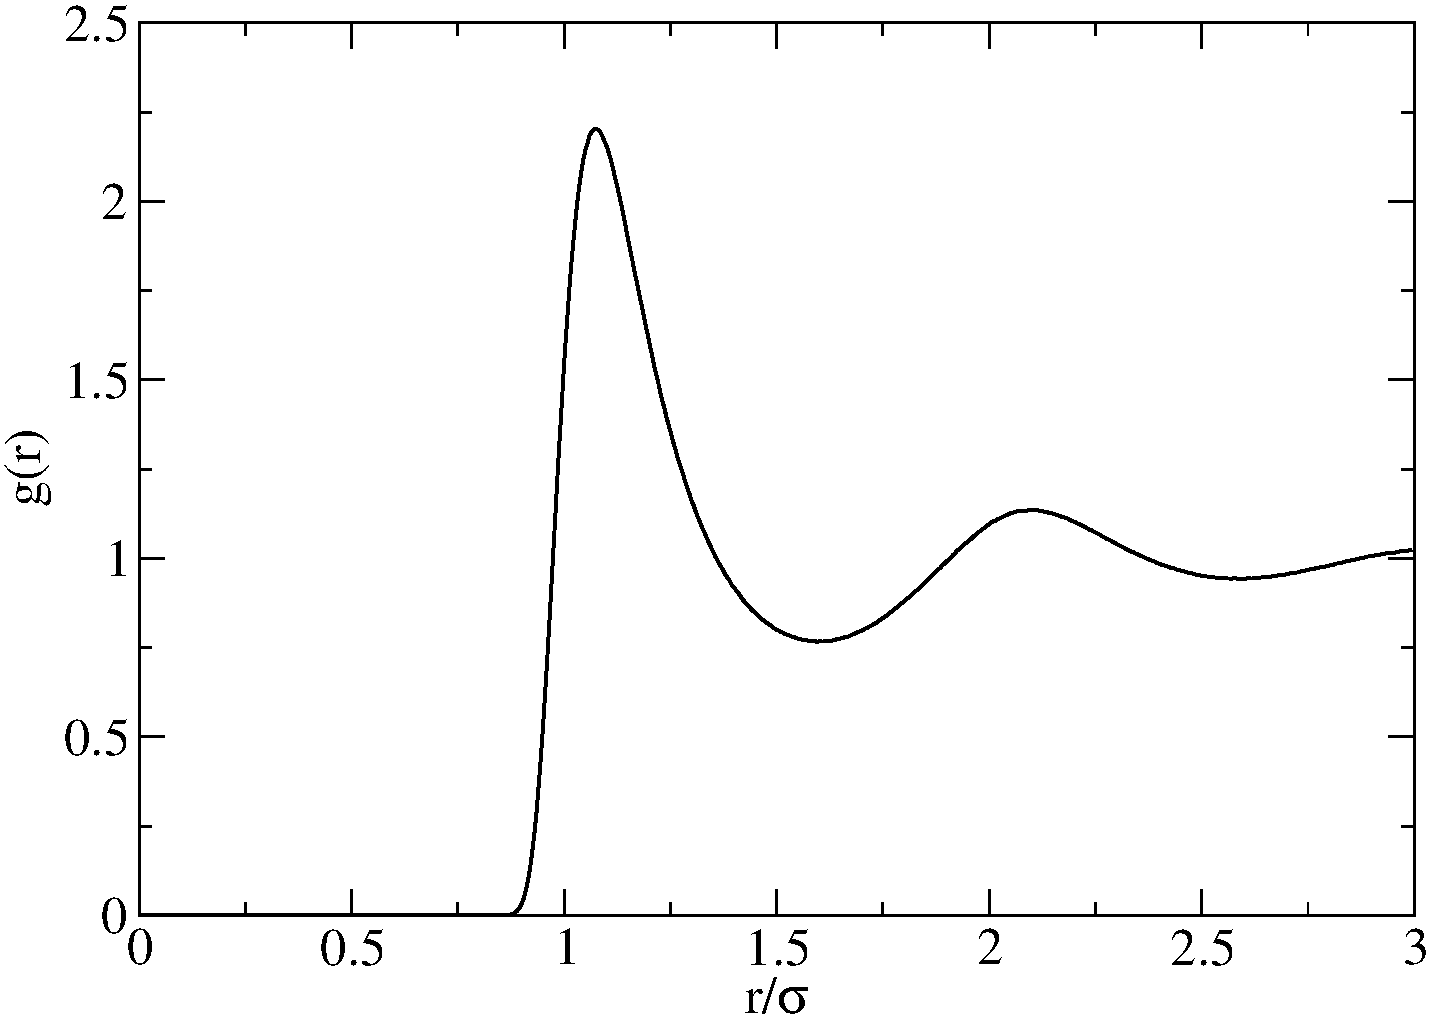
\includegraphics[clip,scale=0.45]{figures/rdfsmooth} 
    \caption[Plot of the radial distribution function for the
    Lennard-Jones density]
    {\label{fig:rdfsmooth} Plot of the radial distribution function,
      $g(r)$, for a continuous Lennard-Jones potential. Results taken
      from a force-driven simulation at $\rho^*=0.7$ and $T^*=1.5$.}
  \end{center}
\end{figure}
\nomenclature[F]{$g(r)$}{Radial distribution function}
The RDF is measured in MD simulations by splitting the radial distance
into a number of bins.  The number of pairs of particles in a
particular bin is then counted.  The value of the RDF for bin $n$ can
be calculated using the following equation:

\begin{equation}
  \label{eq:rdf}
  g(n) = \frac{N_n}{NV_{\text{bin}}\rho}
\end{equation}
where $V_{\text{bin}}$ is the volume of the bin, and $N_n$ is the
number of particle pairs in bin $n$.  This measurement illustrates
another definition of the RDF.  The radial distribution function is
the ratio between the density at a specific distance from another
particle to the average density of the system.

Since the RDF contains information about the potential, simulations
with discrete potentials produce radial distribution functions with
discontinuities in them. Fig.~\ref{fig:rdfrough} shows the RDF
produced when using the stepped potential shown in
Fig.~\ref{fig:chapelasteps}.

\begin{figure}[htp] 
  \begin{center}
    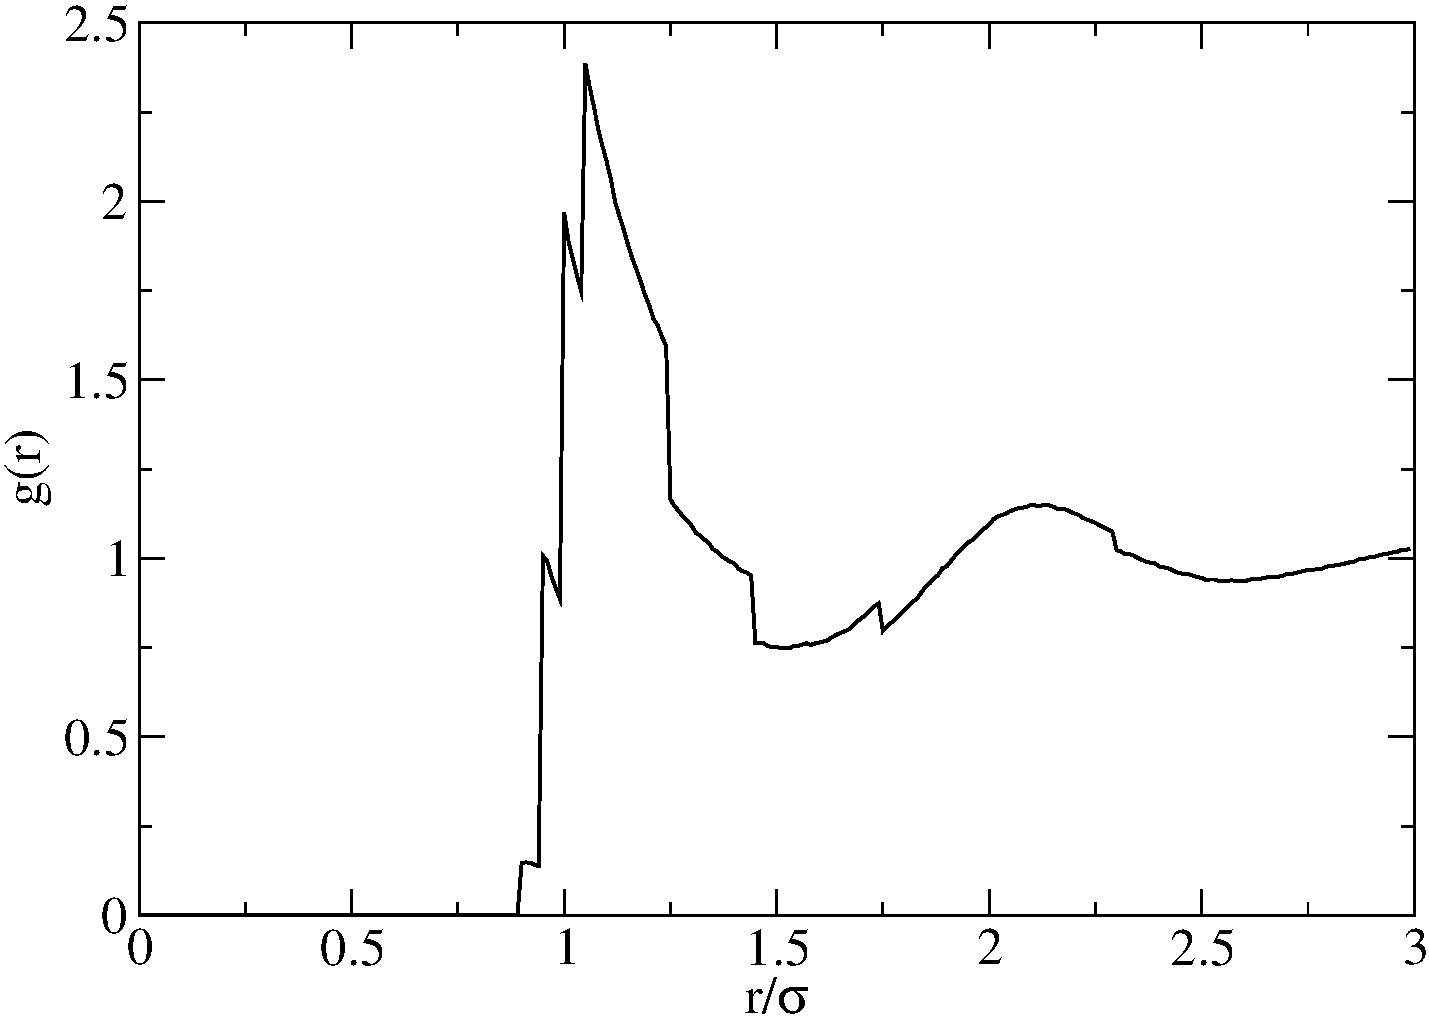
\includegraphics[clip,scale=0.45]{figures/rdfrough} 
    \caption[Plot of the radial distribution function for a discrete
    stepped potential]
    {\label{fig:rdfrough} Plot of the radial distribution
      function, $g(r)$, for a discrete stepped potential. Results
      taken from a event-driven simulation at $\rho^*=0.7$ and $T^*=1.5$.}
  \end{center}
\end{figure}

This discontinuous RDF can be converted to a continuous function by
using the indirect correlation function, $y(r)$,~\cite{Chapela1989}.
The indirect correlation function can be defined for both continuous
and discontinuous RDF and potentials using:

\begin{equation}
  \label{eq:ICF}
  y(r) = g_d(r)e^{\beta\Phi_d(r)} = g_c(r)e^{\beta\Phi_c(r)}
\end{equation}
\nomenclature[F]{$y(r)$}{Indirect Correlation Function}
where $\beta = 1/k_BT$ and the subscripts $c$ and $d$ denote the
continuous and discontinuous functions respectively.  The continuous
form of the RDF can then be calculated using
Eq.~\eqref{eq:continuousRDF}.  Fig.~\ref{fig:rdfcomp} shows the
continuous form of the discontinuous RDF shown in
Fig.~\ref{fig:rdfrough}.

\begin{equation}
  \label{eq:continuousRDF}
  g_c(r)=g_d(r)e^{[\Phi_d(r)-\Phi_c(r)]\beta}
\end{equation}

\begin{figure}[htp] 
  \begin{center}
    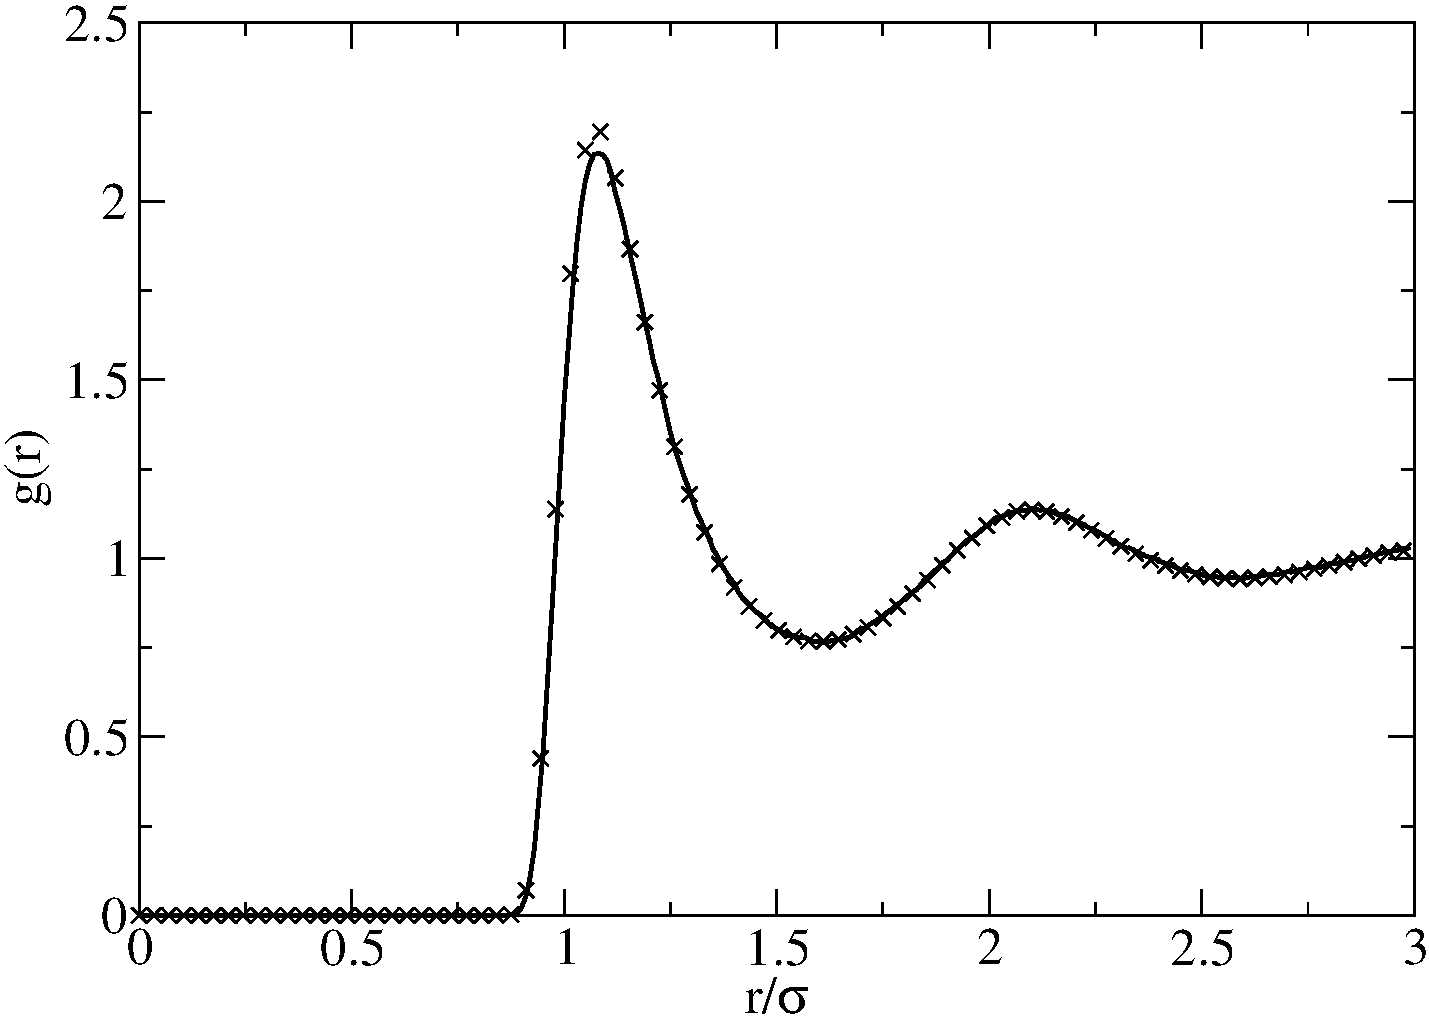
\includegraphics[clip,scale=0.45]{figures/rdfcomp} 
    \caption[Continuous conversion of a discrete radial distribution
    function]
    {\label{fig:rdfcomp} The continuous form of the radial
      distribution function of a discrete potential is shown with the
      solid line.  The crosses show the RDF obtained from the
      continuous Lennard-Jones potential.  Both were obtained at
      $\rho^*=0.7$ and $T^* = 1.5$.}
  \end{center}
\end{figure}

\section{Measuring Properties using the Radial Distribution Function}
\label{sec:RDFMeasure}
Another reason why the radial distribution functions is so important
is that it can be used to calculate other thermodynamic properties.
Any pair function can be related to the RDF ~\cite{Allen1987}, but the
two most important are the potential energy and the pressure, which
can be related to the RDF using Eqs.~\eqref{eq:potentialRDF} and
\eqref{eq:pressureRDF} respectively.

\begin{equation}
  \label{eq:potentialRDF}
  \Phi = 2 \pi \rho N \int^\infty_0 \Phi(r)g(r)r^2 {\rm d}r
\end{equation}

\begin{equation}
  \label{eq:pressureRDF}
  P = \rho k_BT + \frac{2\pi}{3}\rho^2 \int^\infty_0rF(r)g(r)r^2 {\rm d}r
\end{equation}

However, in MD simulations these properties are usually measured using
the methods discussed in Secs.~\ref{sec:Energy}
and~\ref{sec:Pressure} as these are usually more accurate.  

\section{Long-Range Corrections}

In Sec.~\ref{sec:Optimisation}, the truncation of the potential to
increase simulator performance was discussed.  While particles far
apart exert little force between each other, the contributions to the
thermodynamic properties can still be significant.  Therefore it is
common in MD simulations to account for the truncated potential by
adding on a long-range correction.

These long range corrections can be calculated using
Eqs.~\eqref{eq:potentialRDF} and \eqref{eq:pressureRDF}.  Since the
RDF tends to one as separation distance tends to infinity, $g(r)$ is
assumed to be one in these corrections.  Similarly since the
potential, $\Phi(r)$, and the force, $F(r)$, tend to zero as $r$
increases, these are assumed to be zero.  Making these assumptions and
by splitting the integrals Eqs.~\eqref{eq:potentialRDF} and
\eqref{eq:pressureRDF} can be integrated to give equations:

\begin{equation}
  \label{eq:potentialLR}
  \Phi = \Phi_{\text{MD}}+ \frac{8 \pi \rho}{3r_c^3}\left(\frac{1}{3r_c^6} - 1\right)
\end{equation}

\begin{equation}
  \label{eq:pressureLR}
  P = P_{\text{MD}}+ \frac{16 \pi \rho^2}{3r_c^3}\left(\frac{2}{3r_c^6} - 1\right)
\end{equation}
where $r_c$ is the truncation radius of the potential, and the
subscript MD denotes the property measurement from the MD simulation.
These give the long-range corrections for the potential energy and the
pressure respectively.

\section{Units}

In molecular dynamics simulations, properties are frequently measured
in dimensionless forms~\cite{Haile1997}. These ``reduced units'' are
usually denoted with an asterisk.  In order to achieve this a number
of fundamental dimensions are needed: a characteristic length
$\sigma$, a characteristic energy $\varepsilon$, and the mass of one
particle $m$.  In the case of the Lennard-Jones potential, the
characteristic length and energy are taken as the distance of the
root, and the depth of the attractive well respectively. A list of
reduced forms are given in Table~\ref{tab:reducedForms}.
\nomenclature[S]{$x^*$}{Reduced quantity}
\begin{table}[htp] 
  \caption[Table of reduced quantities]
  {Table of reduced forms of various quantities used in this
    dissertation~\cite{Haile1997}.}
  \label{tab:reducedForms}
  \begin{center}
    \begin{tabular}{c c}
      \toprule
      Quantity & Reduced forms \\
      \midrule
      Density & $\rho^* = N \sigma^3 / V$ \\
      Energy & $U^* = U / \varepsilon$ \\
      Force & $F^* = F\sigma/\varepsilon$ \\
      Length & $r^* = r / \sigma$ \\
      Pressure & $P^* = P \sigma^3 /\varepsilon$ \\
      Temperature & $T^* = kT/\varepsilon$ \\
      Time & $t^* = t / (\sigma \sqrt{m/\varepsilon})$ \\
      Velocity & $v^* = v\sqrt{m/\varepsilon}$ \\
      \bottomrule
    \end{tabular}
  \end{center}
\end{table}


\printbibliography[heading=thesisChapterBib] 

\chapter{Converting Continuous Potentials to Discrete Potentials}
\label{chap:cont2dis}
In the previous chapters the tools required to test the effectiveness
of a potential conversion algorithm were discussed.  This chapter will
describe the methods for converting continuous to discrete potentials
that were tried in this 

\section{Introduction}
Discontinuous potentials have a number of desirable properties.  Due
to the analytical nature of event-driven simulation (see
Sec.~\ref{sec:EDIntro}), discontinuous potentials can be solved
precisely, eliminating the errors and instability inherent to
integrators. It is also possible to theoretically derive the equation
of state for a discrete potential fluid using thermodynamic
perturbation theory.

There is, however, a major problem that limits the impact discrete
potentials have had to molecular dynamics.  Firstly, event-driven
simulators are significantly more complex to implement which reduces
the usage of discrete potentials in the literature.  This means while
there are many advanced continuous potentials available, discrete
potentials still remain relatively basic.

If a general method to convert continuous potentials to equivalent
discrete potentials could be developed this would allow the large
number of continuous potentials in the literature to be incorporated
into discrete molecular dynamics.

There are two parameters that need to be decided in order to create a
stepped potential: the placement of the steps; and the energy (or
height) of the steps.  The setting of these parameters will be
discussed in the following sections

\section{Setting Step Positions}

\subsection{Stepping in Even Probability }
\label{sec:probstep}
The first method that was tried was to step in equal probabilities of
a particle being at a certain location.  This should mean there are
more steps at locations where there are more particles. Setting step
positions in probability is equivalent to setting steps in even values
of the partition function. The partition function~\cite{Landau1968}
for a pair of particles is given by:
\begin{equation}
  Z(r_n, r_{n+1}) = 4\pi\int^{r_{n+1}}_{r_n}e^{-\beta\Phi(r)}r^2{\rm d}r 
  \label{eq:partition}
\end{equation}
\nomenclature[F]{$Z$}{Partition function}
\nomenclature[V]{$\beta$}{Reciprocal of the reduced temperature}
where, $r_n$ denotes the position of the $n^{th}$ step and $\beta =
1/T^*$.  By starting at $r_1=r_\text{core}$ the
position of the other steps can be found by solving:
\begin{equation}
  Z(r_n, r_{n+1}) = \frac{Z(r_{\text{core}}, r_{\text{cutoff}})}{N_s}
  \label{eq:probstep}
\end{equation}
for $r_{n+1}$ over the number of steps, $N_s$, until
$r_{n+1}=r_{\text{cutoff}}$.  The solution to Eq.~\eqref{eq:probstep}
is problematic as the variable is a limit of an integral.  This was
solved using a bisection method while the integral was calculated
using Simpson's Rule.

\subsection{Stepping in the Magnitude of the Expected Force}
\label{sec:actionstep}
Though stepping in even probability makes some sense, it makes the
invalid assumption that particles at any position make the same
contribution to system properties.  This is not the case as particles
close together experience a higher force and hence make significant
contributions to the pressure and potential energy of the system.
Therefore the stepping method must taken into account not just the
number of particles but some measure of the effect, such as the force.
The problem with using the force is that can be both positive or
negative which makes stepping in equal values of it impractical.
Therefore the magnitude of the force is used to create
Eq.~\eqref{eq:action}.

\begin{equation}
F_E(r_n, r_{n+1}) = 4\pi \int^{r_{n+1}}_{r_n}|F(r)|e^{-\beta\Phi(r)}r^2{\rm d}r 
\label{eq:action}
\end{equation}

Stepping in equal values of Eq.~\eqref{eq:action} is achieved in a
similar manner to even probability in the preceding section using
Eq.~\eqref{eq:actionstep}.

\begin{equation}
  F_E(r_n, r_{n+1}) = \frac{F_E(r_{\text{core}}, r_{\text{cutoff}})}{N_s}
  \label{eq:actionstep}
\end{equation}
\nomenclature[F]{$F_E$}{Magnitude of the Expected Force}
\subsection{Setting the Position of the Hard Core}
\label{sec:BHcore}
Neither of the two above methods set a suitable location for a hard
core.  All stepped potentials need a hard core to prevent particles
from entering each other, where there is no force to push them apart.

A two methods are considered to define $r_{\text{core}}$.  The
first is to use the Barker-Henderson equivalent hard sphere diameter
\cite{Barker1967a}: 

\begin{equation}
 r_{\text{core}}=\int^{\sigma}_{0}\left(1-e^{\beta\Phi(r)}\right){\rm d}r
\end{equation}

The second is to place the core where there is a very low probability
of particles getting there.  This can be done using the partition
function similar to Sec.~\ref{sec:probstep} using:
\begin{equation}
  Z(0, r_{\text{core}}) = P_{\text{core}}Z(0, r_{\text{cutoff}})
  \label{eq:probcore}
\end{equation}
where $P_{\text{core}}$ is the desired probability of particles reaching the core.

Now that the methods for setting the positions of the steps, the next
section will describe the methods for setting the heights of the steps.
\section{Setting Step Energies}
\label{sec:stepHeight}
\subsection{Setting Heights to Fix Probabilities}
\label{sec:eqProb}
The heights of the steps can be set to ensure the partition function
is the same for both continuous and discrete potentials.
Equation~\eqref{eq:partition} can be integrated over a discrete step
to give:

\begin{equation}
  Z(r_n, r_{n+1}) = \frac{4\pi}{3}\left(r_{n+1}^3 - r_{n}^3\right)e^{-\beta\Phi_n} 
  \label{eq:disPartition}
\end{equation}
where $\Phi_n$ is the height of the step, $n$, that lies from $r_n
\rightarrow r_{n+1}$. This must be equal to the continuous partition
function therefore by equating Eqs.~\eqref{eq:partition} and
\ref{eq:disPartition} an expression can be created for the height of a
single step (Eq.~\eqref{eq:probheight}).

\begin{equation}
  \label{eq:probheight}
  \Phi_n= -\beta^{-1}\ln{\left(\frac{3}{r_{n+1}^3 - r_{n}^3}
      \int^{r_{n+1}}_{r_n}e^{-\beta\,\Phi(r)}\,r^2{\rm d}r\right)}
\end{equation}

Setting the step energies to ensure agreement between the
probabilities of both continuous and discrete potentials should also
ensure that the second virial coefficient is the same.  If a similar
series of steps as above were to be carried out on
Eq.~\eqref{eq:secondVirial2} an identical result to
Eq.~\eqref{eq:probheight} would be obtained.

\begin{equation}
  \label{eq:secondVirial2}
  B_2(r_n, r_{n+1}) = -2\,\pi \int^{r_{n+1}}_{r_n} \left(e^{-\beta\,\Phi(r)}-1\right)r^2{\rm d}r
\end{equation}
\subsection{Setting Heights to Fix Potential Energy}
The expected value for the potential energy between two particles is
the probability of a particle multiplied by the potential energy
integrated over the position.  This means that the expected potential
energy is given by:

\begin{equation}
  \label{eq:energyheight}
  \langle\Phi\rangle^{r_{n+1}}_{r_n} = 4\,\pi\,Z^{-1}(r_n, r_{n+1})
  \int^{r_{n+1}}_{r_n}\Phi(r)e^{-\beta\Phi(r)}r^2{\rm d}r 
\end{equation}
This expected energy over a single discrete step is simply the energy
of the step.  This allows the setting of the heights to ensure the
potential energy of the system is the same in both continuous and
discrete.

A number of techniques to create a general method to convert between
continuous and discrete potentials have been outlined in this section.
It should be noted that many of the expressions in this chapter make
the assumption that the RDF, $g(r)=1$.  This is necessary to derive
these equations but is a strictly invalid assumption.  In the next
chapter these techniques are tested and compared to continuous
potential results to investigate which combination of techniques
produces the most similar stepped potential.

\printbibliography[heading=thesisChapterBib]
\chapter{Results and Discussion}

All the tools and techniques needed to compare a discrete and
continuous potential have been discussed.  In this chapter, the
simulators created for this work will be validated against other
simulators and literature values to ensure that they function
correctly.  Then, all the stepping techniques described in the previous
section will be tested and the best methods will be combined to
produced a general stepping method. Finally, steps produced by this
method will be compared to the steps obtained by Chapela \textit{et
  al.}~\cite{Chapela1989}.

\section{Benchmarking} 

\subsection{Force-Driven Simulator}
The results from the force-driven simulation were checked against a
publicly available force-driven simulation, called ESPResSo
\cite{Limbach2006}.  Simulations were run at $T^*=1.5$ for 50000
time-steps using 864 particles. Measurements were taken every 10
time-steps for the last 30000 steps of the simulation. The mean and
standard deviations of the results of ten simulation runs are shown in
Table~\ref{tab:MDvsEsp}. Very good agreement is shown between all
values with deviations falling inside standard deviations.

\begin{table}[htp]
  \caption[Force-driven simulator benchmarking results]
  {Comparison of results obtained by the force-driven simulator 
    coded for this dissertation and the publicly available simulator, 
    ESPResSo. The numbers in brackets show the standard deviation in 
    the last digit.}
  \label{tab:MDvsEsp}
  \begin{tabular} {l c c c c c c}
    \toprule
    $\rho^*$ & \multicolumn{2}{c}{$\langle T^*\rangle$} 
    & \multicolumn{2}{c}{$\langle P^*\rangle$} 
    & \multicolumn{2}{c}{$\langle\Phi^*\rangle$} \\
    \cmidrule(rl{0.75em}){2-3} 
    \cmidrule(rl{0.75em}){4-5}
    \cmidrule(rl{0.75em}){6-7}
    & Simulator & ESPResSo & Simulator & ESPResSo & Simulator & ESPResSo \\
    \midrule
    0.1 & 1.499(2) & 1.500(4) & 0.1224(3) & 0.1227(5) & -0.708(3)  & -0.705(2)\\
    0.2 & 1.499(2) & 1.500(4) & 0.2069(7) & 0.207(1)  & -1.360(9) & -1.366(5)\\
    0.3 & 1.499(2) & 1.501(2) & 0.280(1)  & 0.282(2)  & -1.975(5) & -1.979(5)\\
    0.4 & 1.499(1) & 1.500(2) & 0.379(4)  & 0.377(3)  & -2.568(5) & -2.569(3)\\
    0.5 & 1.499(2) & 1.500(3) & 0.567(5)  & 0.568(5)  & -3.164(3) & -3.165(3)\\
    0.6 & 1.500(2) & 1.500(4) & 0.988(6)  & 0.988(9)  & -3.771(1) & -3.774(2)\\
    0.7 & 1.499(1) & 1.501(3) & 1.894(5)  & 1.90(1)   & -4.358(2) & -4.360(2)\\
    0.8 & 1.499(2) & 1.498(2) & 3.68(1)   & 3.68(1)   & -4.869(2) & -4.872(2)\\
    0.9 & 1.499(1) & 1.501(3) & 6.88(1)   & 6.90(2)   & -5.227(2) & -5.226(4)\\
    \bottomrule
  \end{tabular}
\end{table}
\subsection{Event-Driven Simulator}

Due to the complex nature of event-driven simulations the benchmarking
was split into two tests.
\begin{flushleft}
\textbf{Testing Hard Spheres}
\end{flushleft}
The event-driven simulator was first tested running a hard sphere
simulation before testing the more complex stepped potentials. A
single 'step' with a energy requirement sufficiently large such that
no particle could enter it. The simulation was run once at a range of
densities using 864 particles at a reduced temperature of $T^*=1$ for
5 million collisions, the results were compared with those of
Lue~\cite{Lue2005} in Table~\ref{tab:benchhard}. The agreement between
results is good and lies within statistical uncertainty. The largest
discrepancies are in the values for the coefficient of diffusion at
low densities which is probably due to Lue's values were obtained
after 10 million collisions which is longer than the 5 million
collisions run by the event-driven simulator.

\begin{table} [htp]
  \caption [Event-driven simulation hard sphere benchmarking results]
  {Comparison of results obtained by the
    event-driven simulator with literature values. $t_{avg}$ is the
    average time between collisions, $\langle\mathbf{\hat{r}} \cdot
    \Delta \mathbf{v} \rangle_{coll}$ is the average momentum
    transfer per collision, and D is the coefficient of diffusion.}
  \label{tab:benchhard} 
  \begin{center} 
    \begin{tabular}{l c c c c c c} 
      \toprule $\rho$ & \multicolumn{2}{c}{$t_{avg}$} &
      \multicolumn{2}{c}{$\langle\mathbf{\hat{r}} \cdot \Delta
        \mathbf{v} \rangle_{coll}$} & \multicolumn{2}{c}{D} \\ 
      \cmidrule(rl{0.75em}){2-3} 
      \cmidrule(rl{0.75em}){4-5}
      \cmidrule(rl{0.75em}){6-7} & Simulator & Lue & Simulator & Lue &
      Simulator & Lue
      \\ \midrule 0.3 & 0.3052 & 0.3052 & 1.775 & 1.772 & 0.53 & 0.55 
      \\ 0.4 & 0.1944 & 0.1942 & 1.776 & 1.773 & 0.341 & 0.359 
      \\ 0.5 & 0.13024 & 0.13031 & 1.774 & 1.7724 & 0.247 & 0.247 
      \\ 0.6 & 0.08966 & 0.08968 & 1.771 & 1.7721 & 0.169 & 0.173 
      \\ 0.7 & 0.0625 & 0.0625 & 1.773 & 1.776 & 0.114 & 0.113
      \\ 0.8 & 0.04365 & 0.0436 & 1.772 & 1.772 & 0.064 & 0.065 
      \\ 0.9 & 0.03029 & 0.03024 & 1.773 & 1.772 & 0.033 & 0.0327
      \\ \bottomrule
    \end{tabular} 
  \end{center} 
\end{table}
\begin{flushleft}
\textbf{Testing Step Potentials}
\end{flushleft}
The simulator was then benchmarked using a step potential. The results
were compared with Chapela \textit{et al.}~\cite{Chapela1989} using their 'Case
6' steps. The simulation was run for 1.5 million collisions using 864
particles. Each simulation was run ten times and the mean values and
standard deviations are given in Table~\ref{tab:benchsoft}.

\begin{table} [htp]
  \caption[Event-driven simulation stepped potential benchmarking results]
  {Comparison of results
    obtained by the event-driven simulator with literature values
    using stepped potentials. Numbers in parenthesis indicate the
    standard deviation in the final digit.
    \label{tab:benchsoft}} 
  \begin{center} 
    \begin{tabular}{l c c c c c c} 
      \toprule
      $\rho$ & \multicolumn{2}{c}{$\langle T\rangle$} &
      \multicolumn{2}{c}{$\langle U \rangle$} &
      \multicolumn{2}{c}{$\langle P \rangle$}
      \\ \cmidrule(rl{0.75em}){2-3} \cmidrule(rl{0.75em}){4-5}
      \cmidrule(rl{0.75em}){6-7}& Simulator & Chapela \textit{et al.} &
      Simulator & Chapela \textit{et al.} & Simulator & Chapela \textit{et al.}\\ 
      \midrule
      0.85 & 0.719(3) & 0.72 & -6.04(7) & -5.80 & -0.5(4) & 0.54
      \\ 0.85& 1.339(8) & 1.34 & -5.130(9) & -5.14 & 4.08(4) & 4.08
      \\ 0.85 & 2.35(1) & 2.35 & -4.24(2) & -4.20 & 8.78(9) & 8.86
      \\ 0.85 & 3.37(2) & 3.37 & -3.48(2) & -3.49 & 12.90(9) & 13.00
      \\ 0.85 & 4.59(1) & 4.60 & -2.67(1) & -2.68 & 17.31(8) & 13.43
      \\ 0.75 & 0.811(2) & 0.81 & -5.095(3) & -5.08 & -0.20(2) & -0.24
      \\ 0.75 &1.309(9) & 1.31 & -4.67(1) & -4.63 & 1.81(5) & 1.84
      \\ 0.75 & 2.49(1) & 2.49 & -3.88(1) & -3.82 & 5.80(4) & 5.95
      \\ 0.75 & 3.59(2) & 3.59 & -3.26(1) & -3.22 & 9.03(7) & 9.20
      \\ 0.65 & 1.309(8) & 1.31 & -4.081(8) & -4.06 & 0.80(3) & 0.81
      \\0.65 & 2.61(1) & 2.61 & -3.42(1) & -3.41 & 3.86(5) & 3.89
      \\ 0.65 & 3.79(1) & 3.79 & -2.926(9) & -2.94 & 6.34(7) & 6.33
      \\ 
      \bottomrule 
    \end{tabular}
  \end{center} 
\end{table} 

Again the agreement between the results obtained from the simulator
and those in the literature is good, there are however a few
anomalies.  The results for $\rho^* = 0.85, T^*= 0.72$ and $\rho^* =
0.75, T^*= 0.81$ don't match very well, but this is due to these
points lying in two-phase region which MD simulators don't work overly
well.  The other anomaly is the pressure calculated at $\rho^* = 0.85,
T^*= 4.60$, the value from Chapela \textit{et al.} does not match the
trend and was probably supposed to be $\langle P^* \rangle = 17.43$.
The validity of this data point and confirmation the two-phase
behaviour of the first two anomalies was checked using another
event-driven simulator, DynamO~\cite{Bannerman2011}.  Good agreement
was found between DynamO and this dissertation's event-driven
simulator so these anomalies can be disregarded.

Now that the simulators are confirmed to be functioning correctly,
comparisons can be made between continuous and discrete potentials.
This dissertation will use the Lennard-Jones potential and attempt to
find a suitable method to create an equivalent discrete potential.
First, a comparison will be made with stepping methods already
developed in the literature.

\section{Previous Stepping Methods}
There have been a number of methods used to convert continuous to
discrete potentials previous to this dissertation.  These discrete
potentials are usually either handmade~\cite{Chapela1989, Unlu2004,
  ElliotJr2002} or simply have the steps placed at even
intervals~\cite{Chapela2010}.  Since Chapela \textit{et al.} used ten
steps all discrete potentials created in this section will also use
ten steps to allow comparisons to be made.  A set of evenly spaced
steps were created starting from a Barker-Henderson hard core
diameter~\cite{Barker1967a} (see Sec.~\ref{sec:BHcore}) to a cutoff
radius of $3\sigma$.  The cutoff radius value of $3\sigma$ was chosen
as it is the truncation radius used in the force-driven simulation and
all potentials generated in this chapter will use this cutoff.  The
heights of this evenly spaced potential was set so the areas under the
discrete potential were the same as that for the continuous potential.

Figure \ref{fig:prevComp} shows a comparison of results from a
continuous potential to the evenly spaced step potential and the
hand-made potential created by Chapela \textit{et al.}  It can be seen
that evenly spaced steps do not reproduce the continuous potential
results.  

\begin{figure}[htp] 
  \begin{center}
    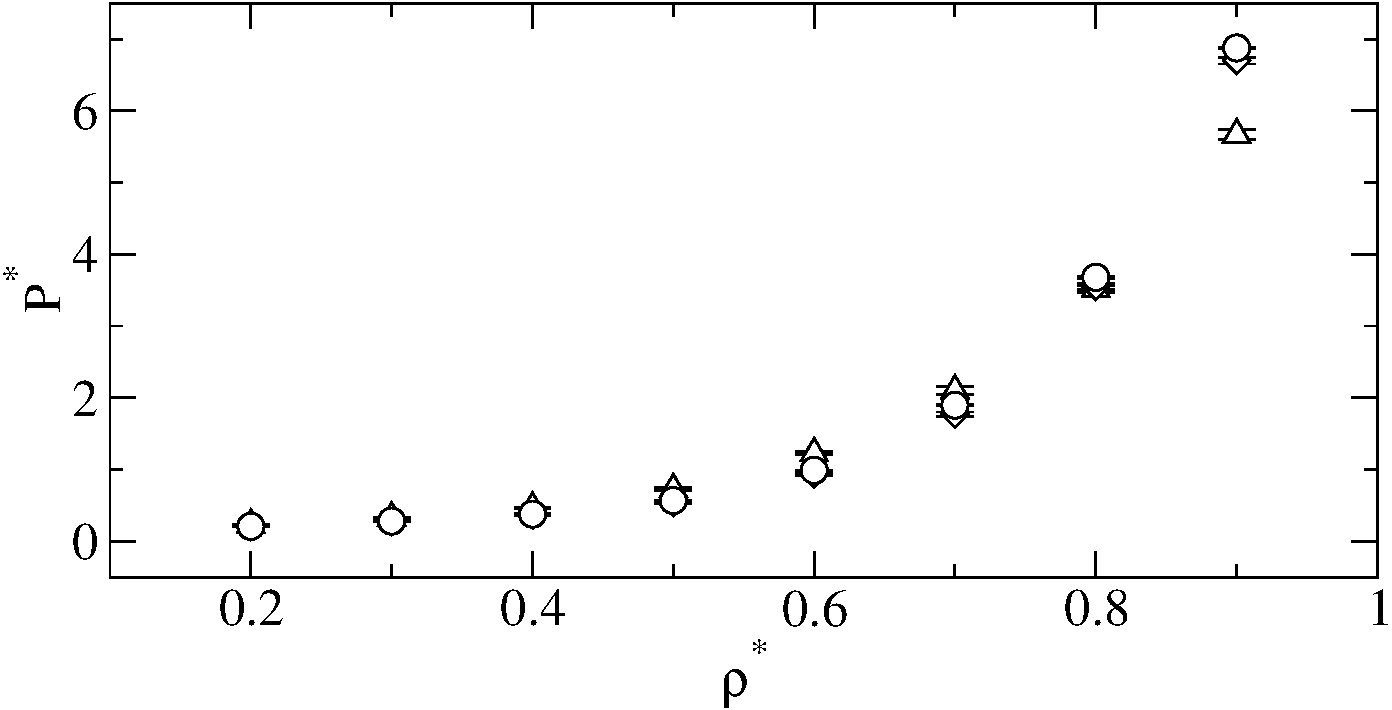
\includegraphics[clip,scale=0.45]{figures/ChapelaP} 
    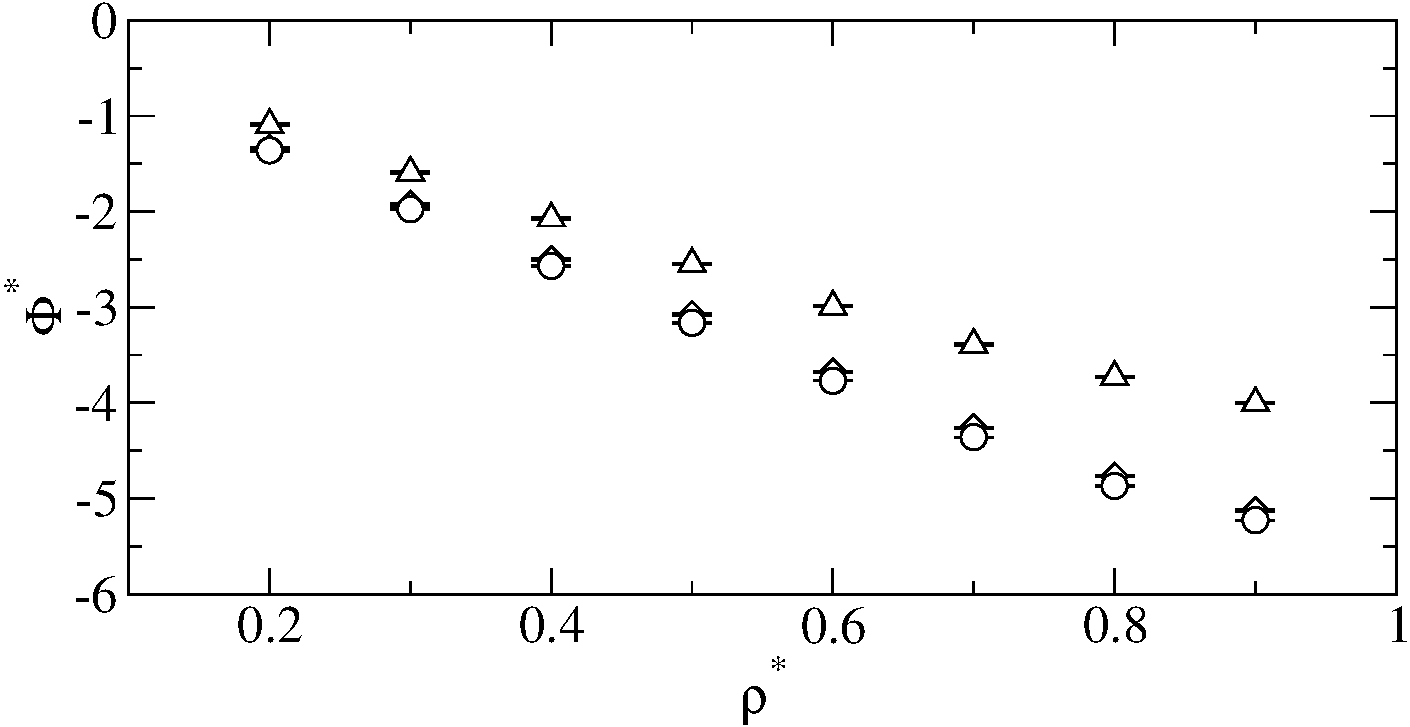
\includegraphics[clip,scale=0.45]{figures/ChapelaU} 
    \caption[Comparison of continuous potential results with existing
    stepping methods] {Plot of the reduced pressure (top) and
      potential energy (bottom) obtained from a continuous potential
      (circle); evenly-spaced steps (triangle); and the handmade steps
      from Chapela \textit{et al.} (diamond).}
    \label{fig:prevComp}
  \end{center}
\end{figure}

The potential from Chapela \textit{et al.} is significantly better and
shows that it is indeed possible to create a stepped potential that
can give similar results to a continuous potential.  The results
plotted here are the results measured using the techniques described
in Secs.~\ref{sec:Energy} and \ref{sec:Pressure}.  Chapela \textit{et
  al.} recommended using results measured from a converted RDF
(Secs.~\ref{sec:RDF} and \ref{sec:RDFMeasure}); however, by doing this
they sacrifice accuracy in pressure for accuracy in potential energy.
As measuring values in the simulation and not from the RDF is more
useful, these are the results that will be used from now on.  

Creating a handmade potential is very time consuming, therefore there
is a need to create an automatic stepping method.  A number of
techniques to create such a method will now be tested to investigate
their effectiveness.

\section{Stepping in Probability Versus Expected Force}

The first method to create a stepped version of the Lennard-Jones
potential was to step in equal probabilities (described in
Sec.~\ref{sec:probstep}), starting with a core step calculated using
the Barker-Henderson equivalent hard sphere diameter . The step
heights were assigned using the equal probability method described in
Sec.~\ref{sec:eqProb}.  The steps produced by this method is shown
in Fig.~\ref{fig:probStepping}.  It can be seen that these steps do not
follow the Lennard-Jones potential very well.  The hard core and base
of the well have been under-stepped.  This is problematic as the core
is fundamental to the freezing behaviour~\cite{Alder1957}, and makes a
large contribution to the pressure.  

\begin{figure}[htp] 
  \begin{center}
    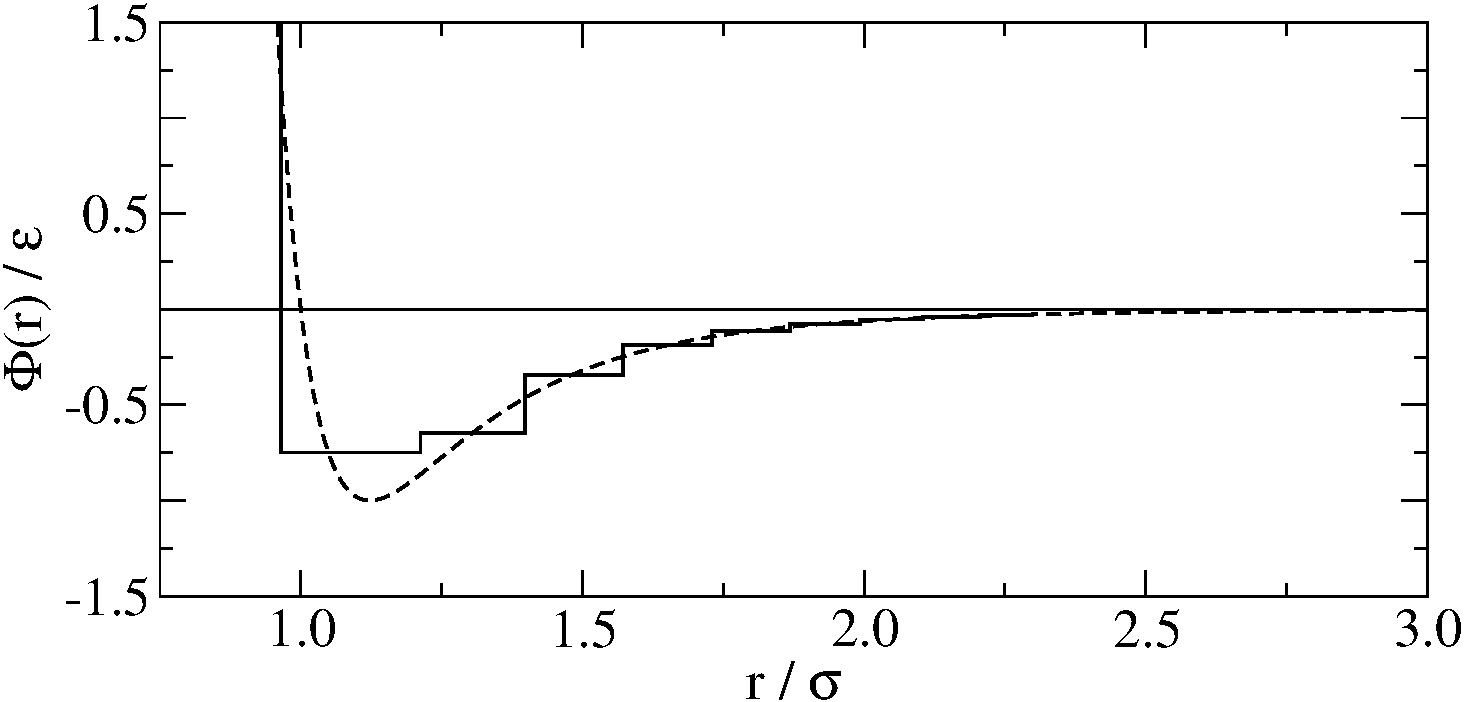
\includegraphics[clip,scale=0.45]{figures/probSteps} 
    \caption[Steps produced using equal probabilities compared with
    continuous potential]
    {Plot of the steps produced by setting step positions in equal
      probabilities (solid) compared with the continuous Lennard-Jones
      potential (dashed).}
    \label{fig:probStepping}
  \end{center}
\end{figure}

\begin{figure}[htp] 
  \begin{center}
    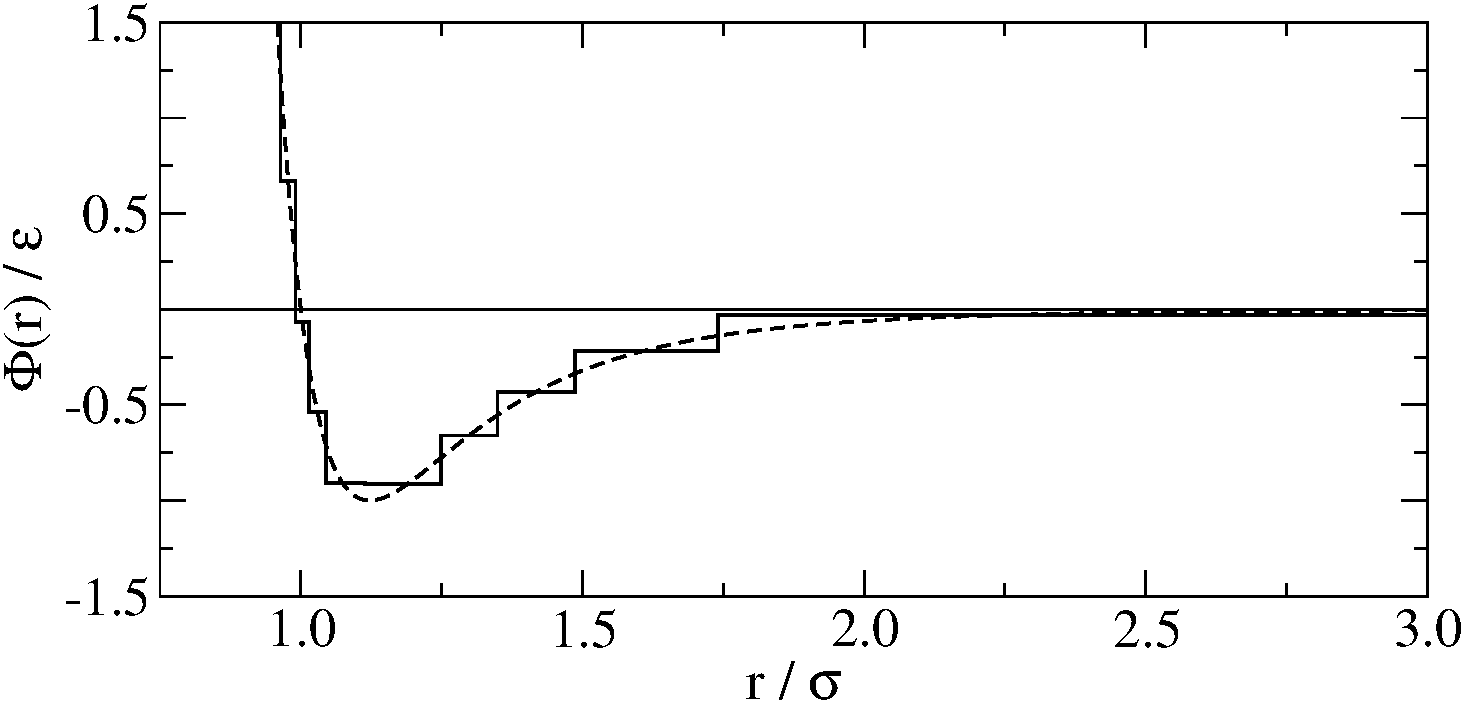
\includegraphics[clip,scale=0.45]{figures/actionSteps} 
    \caption[Steps produced using equal magnitudes of the expected
    force compared with the continuous potential]
    {Plot of the steps produced by setting the step positions in equal
      magnitudes of the expected force (solid) compared with the
      continuous Lennard-Jones potential (dashed).}
    \label{fig:actionSteps}
  \end{center}
\end{figure}
Clearly a better method is needed.  The reason the equal probability
stepping failed is because even though the core is important there are
very few particles there, hence it is under-represented.  What is
needed to improve this is to multiply the probability by a factor that
is high at the core.  The definition of the core is that the force is
nearly infinite so this was used.  This new method, stepping in equal
contributions to the absolute value of the expected force is outlined
in Sec.~\ref{sec:actionstep}.  The steps produced using this method
is shown in Fig.~\ref{fig:actionSteps}. Again the innermost step was
assigned using the Barker-Henderson hard sphere diameter, and the step
heights were assigned to ensure equal probability.  It can be seen
that these steps match the Lennard-Jones potential significantly
better than the probability stepping method.

\begin{figure}[htp] 
  \begin{center}
    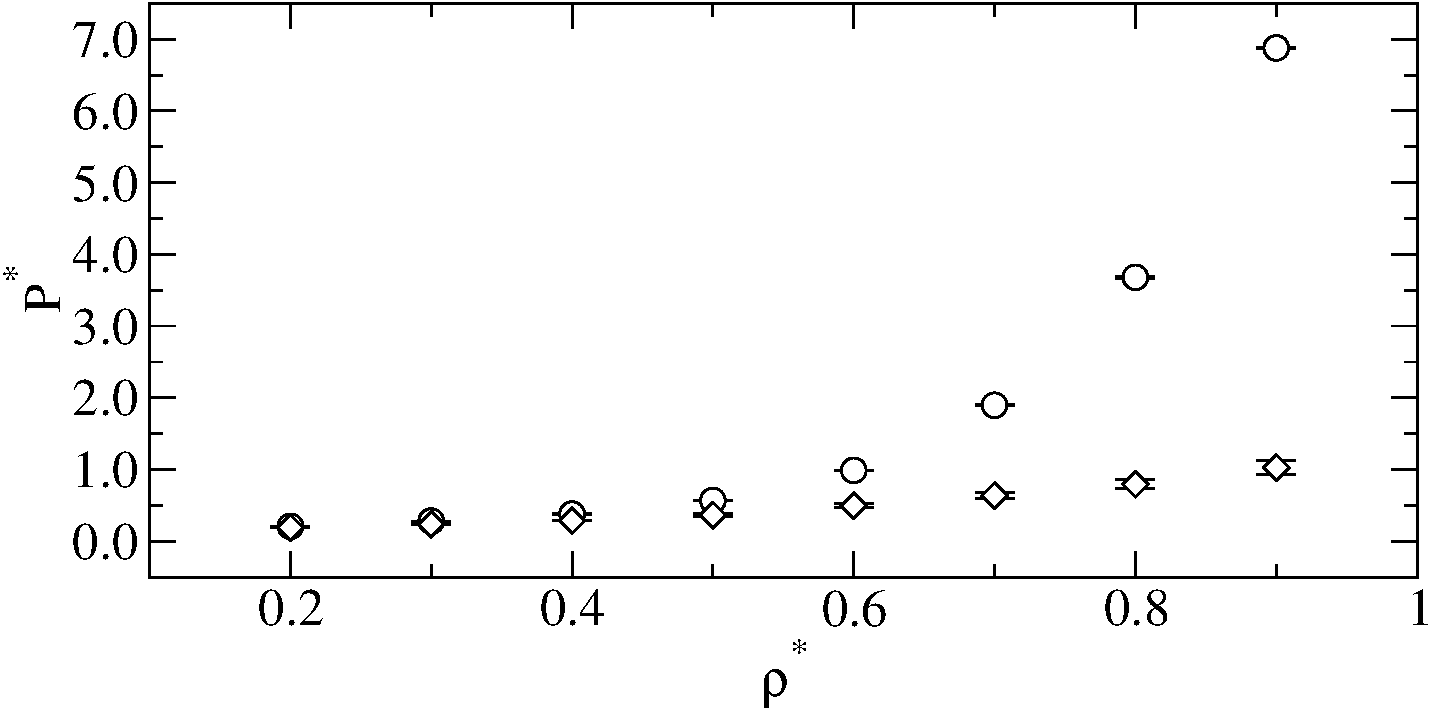
\includegraphics[clip,scale=0.45]{figures/actionNoCoreP} 
    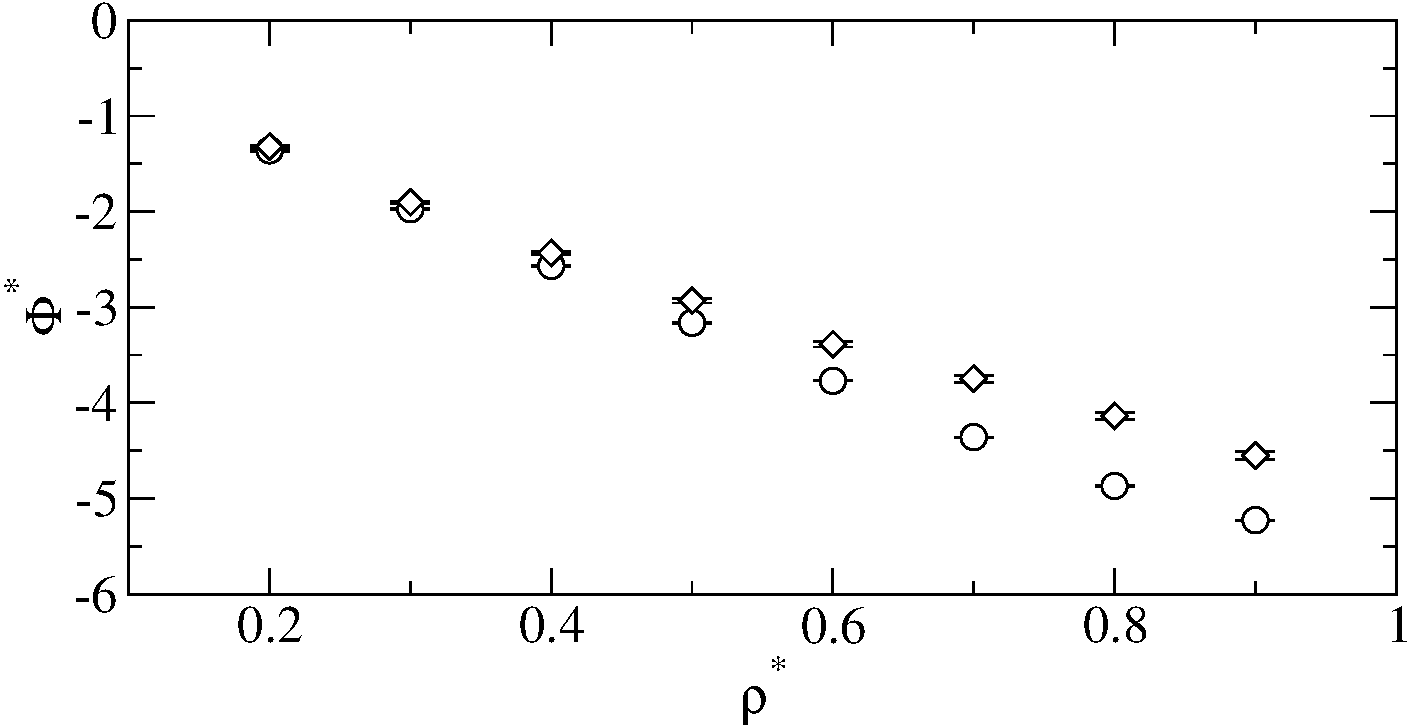
\includegraphics[clip,scale=0.45]{figures/actionNoCoreU} 
    \caption[Comparison of results from a continuous potential and
    those using steps set using the magnitude of the expected force]
    {Plot of the reduced pressure (top) and potential energy (bottom)
      obtained from a continuous potential (circle) and steps set
      using the magnitude of the expected force (diamond).}
    \label{fig:actionNoCore}
  \end{center}
\end{figure}

The results of a simulation run with these steps is shown in
Fig.~\ref{fig:actionNoCore}. As can be seen these steps do not match
the continuous potential results, this is probably due to the hard
core not being repulsive enough to keep the particles out of the core.
This can be seen on the discontinuous RDF (see
Fig.~\ref{fig:noCoreRDF}); there should be no particles inside the
innermost step at $r\approx 0.96\sigma$, but the plot of the RDF
clearly is non-zero well inside the core.


\begin{figure}[htp] 
  \begin{center}
    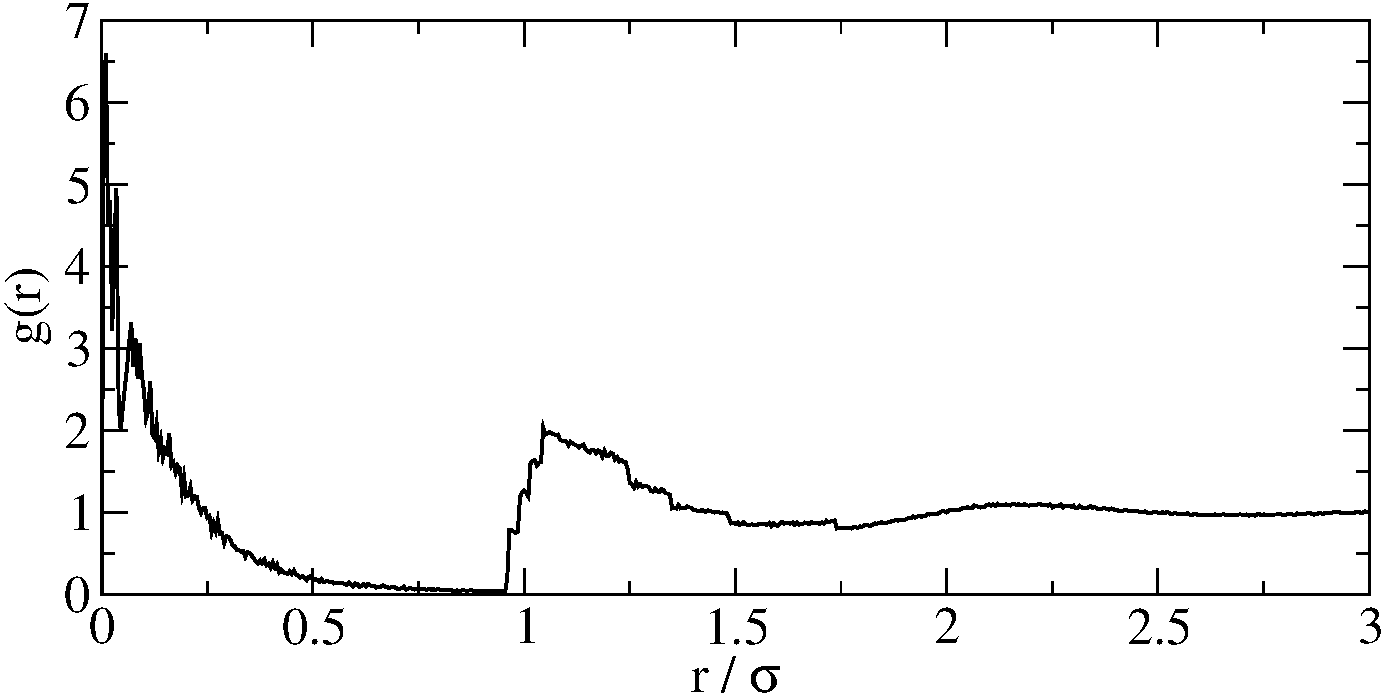
\includegraphics[clip,scale=0.45]{figures/noCoreRDF} 
    \caption{Plot of the RDF of the magnitude of expected force
      stepping without a hard core.}
    \label{fig:noCoreRDF}
  \end{center}
\end{figure}

Therefore this method does not create a sufficiently ``hard'' core to
keep particles outside each other.  In the next, the placement of this
hard core will be investigated

\section{Hard Core Position}

In the previous section, it was discovered that the core was
sufficiently hard to ensure no particles could enter it.  This was
rectified by increasing the energy of the inner core to a very large
value.  

\begin{figure}[htp] 
  \begin{center}
    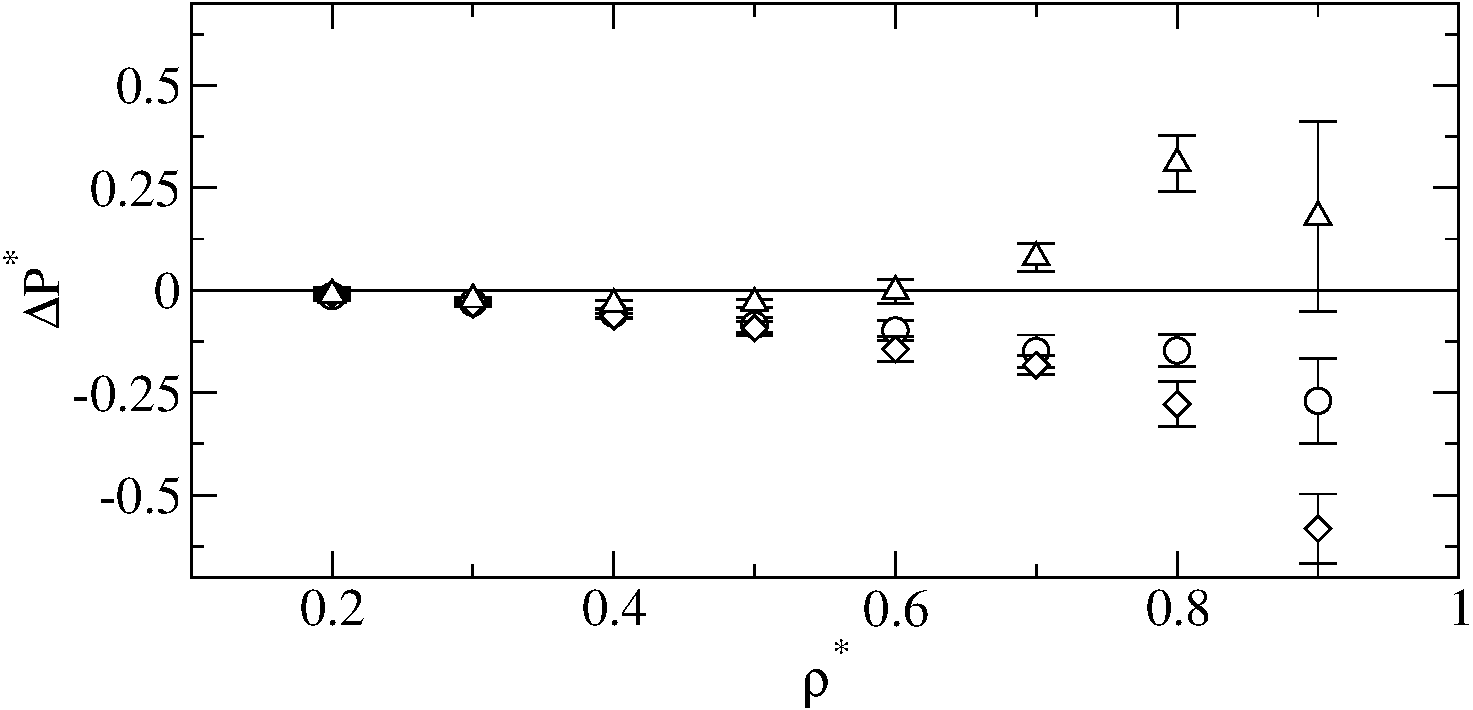
\includegraphics[clip,scale=0.45]{figures/coresP} 
    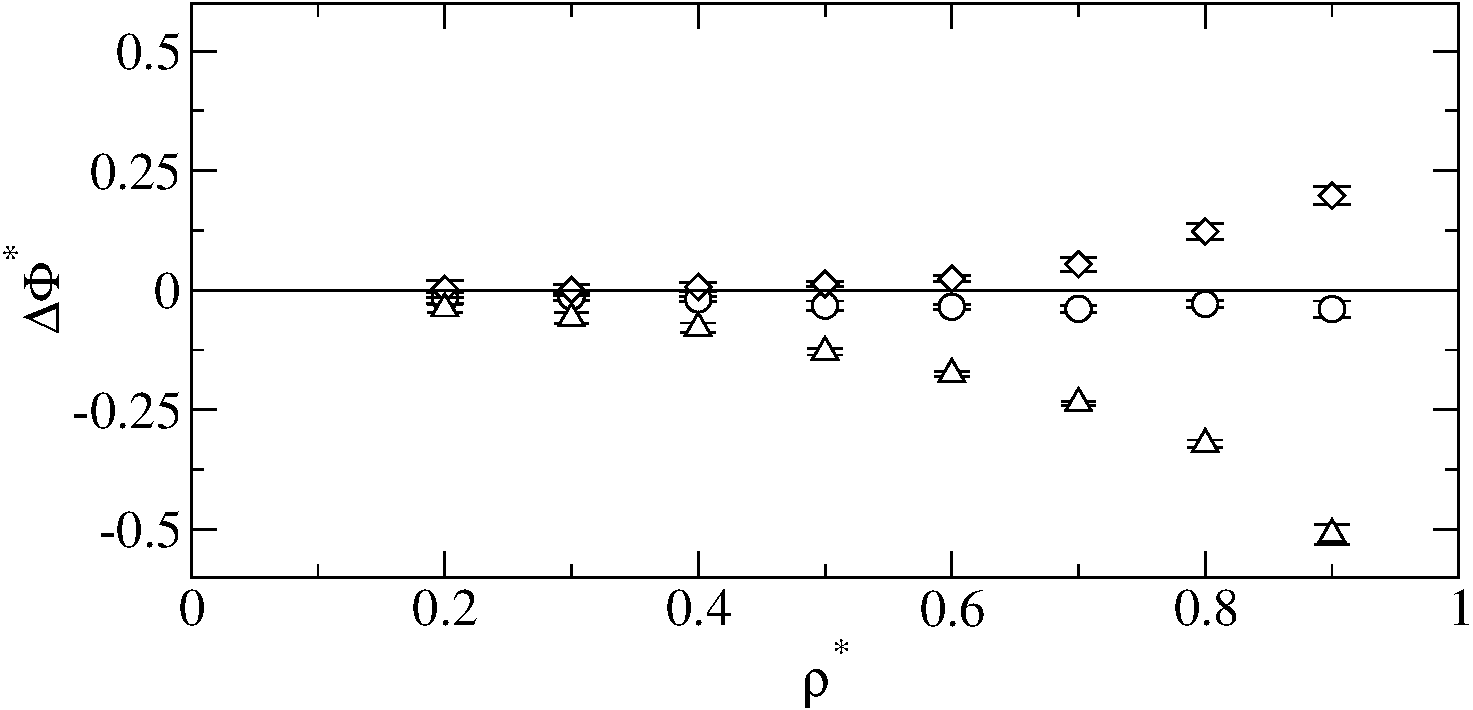
\includegraphics[clip,scale=0.45]{figures/coresU} 
    \caption [Comparison of the errors from the force-driven
    simulation of various hard core placement]
    {Plot of the error in reduced pressure(top) and potential(bottom)
      energy from the force-driven simulation obtained from a hard
      core placed using Barker-Henderson(triangle); $4$ SD (circle);
      and $5$ SD (diamond).}
    \label{fig:compCore}
  \end{center}
\end{figure}

Until now the position of the inner core was selected using the
Barker-Henderson equivalent hard sphere diameter; however, this may
not be the best choice.  The Barker-Henderson hard sphere diameter is
only an approximation and was chosen in this dissertation due to its
simplicity.  An alternative method for selecting the hard core
diameter is described in Sec.~\ref{sec:BHcore}, and it places the
core at a point where very few particles reach.  Cores are placed at
positions where four or five standard deviations (SD) of particles are
located outside of the core.  The results of this comparison is shown
in Fig.~\ref{fig:compCore}.

It can be seen that $4\,\text{SD}$ gives the best results for both pressure
and potential energy, and hence, is the hard core position recommended
by this dissertation.
\section{Investigating Step Height Methods}

A brief comparison was carried out to investigate the best method to
set the heights of the steps.  In Sec.~\ref{sec:stepHeight}, two
methods were suggested to set the heights of the steps: either
ensuring equal probability or equal potential energy.  A set of
steps for each were generated for $T^*=1.5$ with a Barker-Henderson
hard sphere diameter and the heights are shown in Table~\ref{tab:heightcomp}

\begin{table} [htp]
  \caption[Comparison of step energies created by different methods]
  {Comparison of step energies produced by setting heights using probability and energy.}
  \label{tab:heightcomp}
  \begin{center}
    \begin{tabular} {l c c c}
      \toprule
      $n$ & $r_n$ & \multicolumn{2}{c}{$\Phi_n$} \\
      \cmidrule(rl{0.75em}){3-4}
      & & Probability & Energy \\
      \midrule
      1 & 0.964 &  4.761 & 2.086 \\
      2 & 0.991 &  0.658 & 0.633\\
      3 & 1.016 & -0.074 & -0.082 \\
      4 & 1.045 & -0.542 & -0.546 \\
      5 & 1.120 & -0.918 & -0.920 \\
      6 & 1.250 & -0.910 & -0.911 \\
      7 & 1.350 & -0.659 & -0.660 \\
      8 & 1.488 & -0.433 & -0.434 \\
      9 & 1.741 & -0.217 & -0.218 \\
      10& 3.000 & -0.028 & -0.028 \\
      \bottomrule
    \end{tabular}
  \end{center}
\end{table}

There is very little difference in the heights of most of the steps
therefore it is unlikely there is any significant difference between
them.  This was proven by running a simulation of both systems and the
results were very similar.

\section{Comparison with Previous Results}

Now a complete stepping method has been created, it will be compared
to those obtained by Chapela \textit{et al.}
Figure~\ref{fig:ChapelaComp} shows the relative errors from the
continuous potential for both stepping methods.

\begin{figure}[htp] 
  \begin{center}
    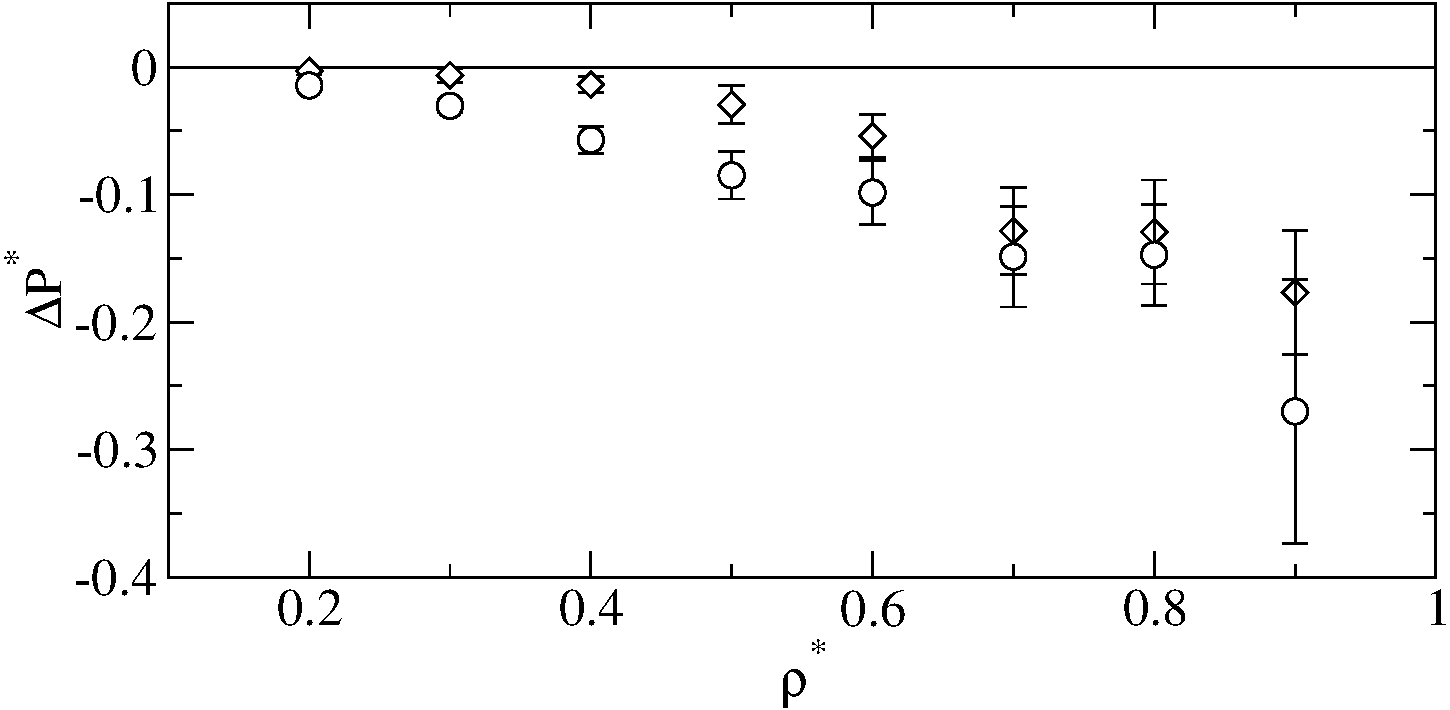
\includegraphics[clip,scale=0.45]{figures/ChapelaCompP} 
    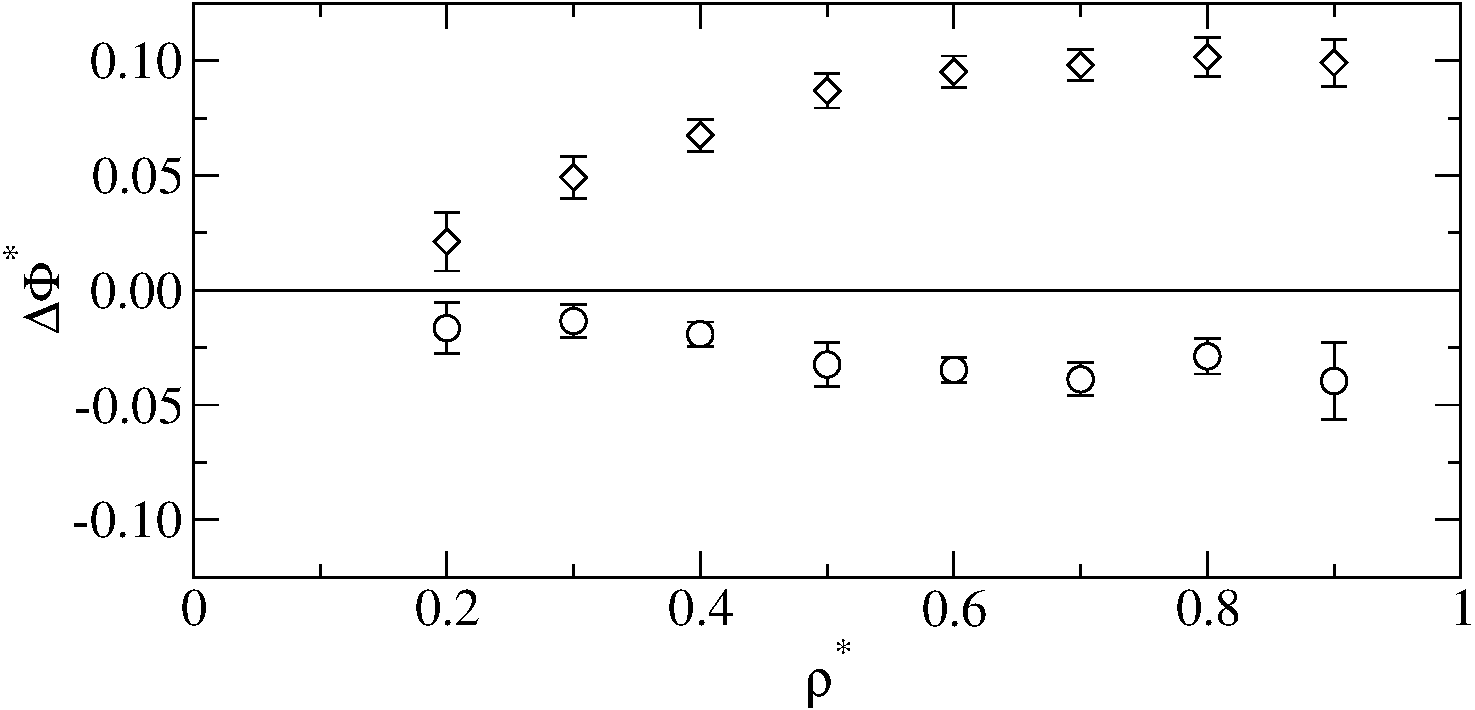
\includegraphics[clip,scale=0.45]{figures/ChapelaCompU} 
    \caption[Comparison of results between previous work and this
    dissertations steps]
    {Plot of the error in the reduced pressure (top) and potential
      energy (bottom) from the continuous potential results for
      magnitude of the expected force steps (circle); and the steps
      from Chapela \textit{et al.} (diamond).}
    \label{fig:ChapelaComp}
  \end{center}
\end{figure}

The potential created by Chapela \textit{et al.} is slightly better
that the one created in this dissertation for the pressure of the
system, with this expected force stepping deviating from the
force-driven simulators results at lower densities.  The potential on
the other hand is far better represented by the expected force
stepping.  The error from the continuous results is fairly constant
with density and much lower than that for Chapela \textit{et al.}  

It should be noted here that the errors in both these stepping methods
are very small when compared to the magnitudes of the values
(Fig.~\ref{fig:prevComp} shows the similarity between Chapela
\textit{et al.} and the continuous potential results).
\section{Temperature Comparisons}
\label{sec:tempcomp}
The advantage of the current stepping system is that all the methods
are dependant on the temperature of the system.  This should mean that
the results of the simulation deteriorate slower than those taken
from Chapela \textit{et al.}.

The error in potential energy from the force-driven simulation at a
number of temperatures is shown in Fig.~\ref{fig:tempU}.

\begin{figure}[htp] 
  \begin{center}
    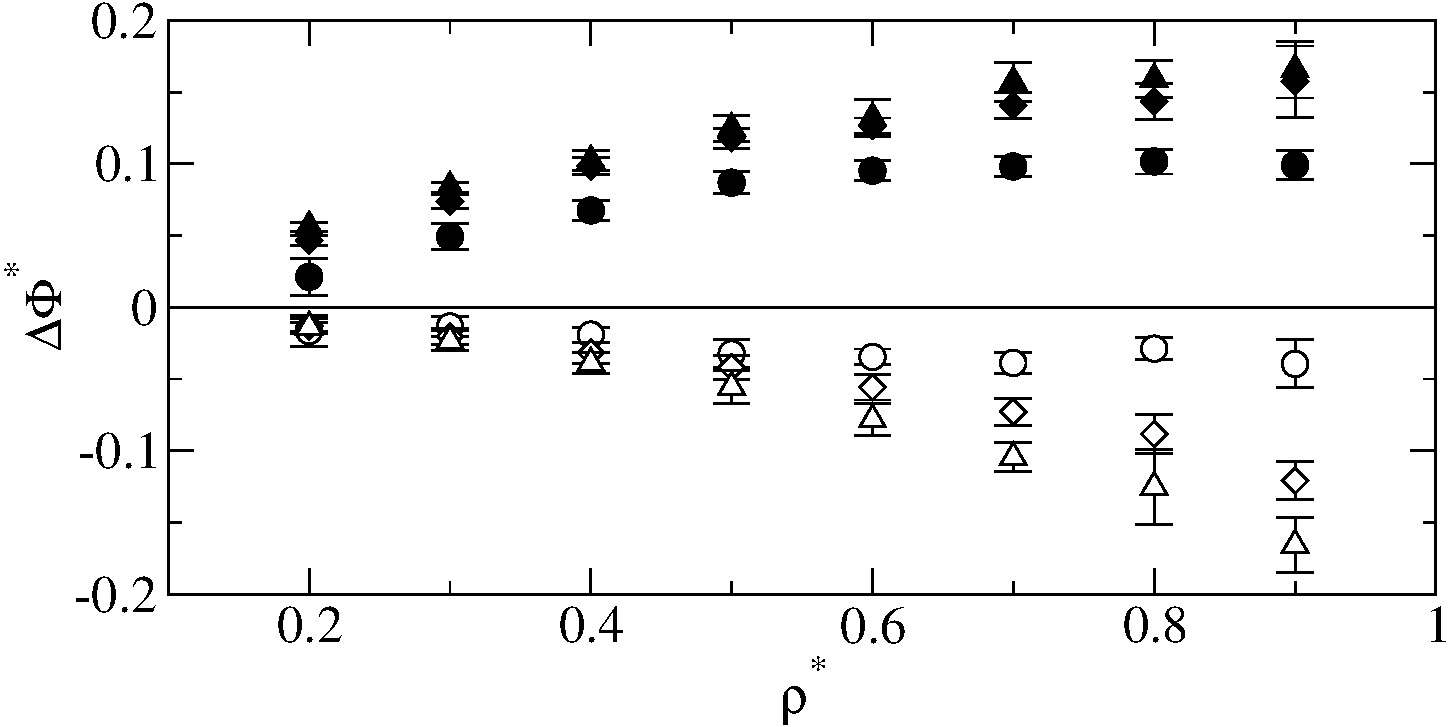
\includegraphics[clip,scale=0.45]{figures/TempU} 
    \caption[Temperature comparison of potential energy between
    previous steps and this dissertations steps]
    {\label{fig:tempU} Temperature comparison of errors in potential
      energy obtained from Chapela \textit{et al.} steps (filled), and
      this dissertation's steps (unfilled) at temperatures of
      $T^*=1.5$ (circle), $T^*=3.0$ (diamond) and $T^*=4.5$
      (triangle).}
    \end{center}
\end{figure}

It can be seen that stepping method developed in this dissertation
actually increases in error faster than potential created by Chapela
\textit{et al.}.  As temperature increases the steps are more densely
concentrated at the inner core which is correct; this implies that it
is the height determining aspect of the stepping method that is to
blame for this deterioration. 

\begin{figure}[htp] 
  \begin{center}
    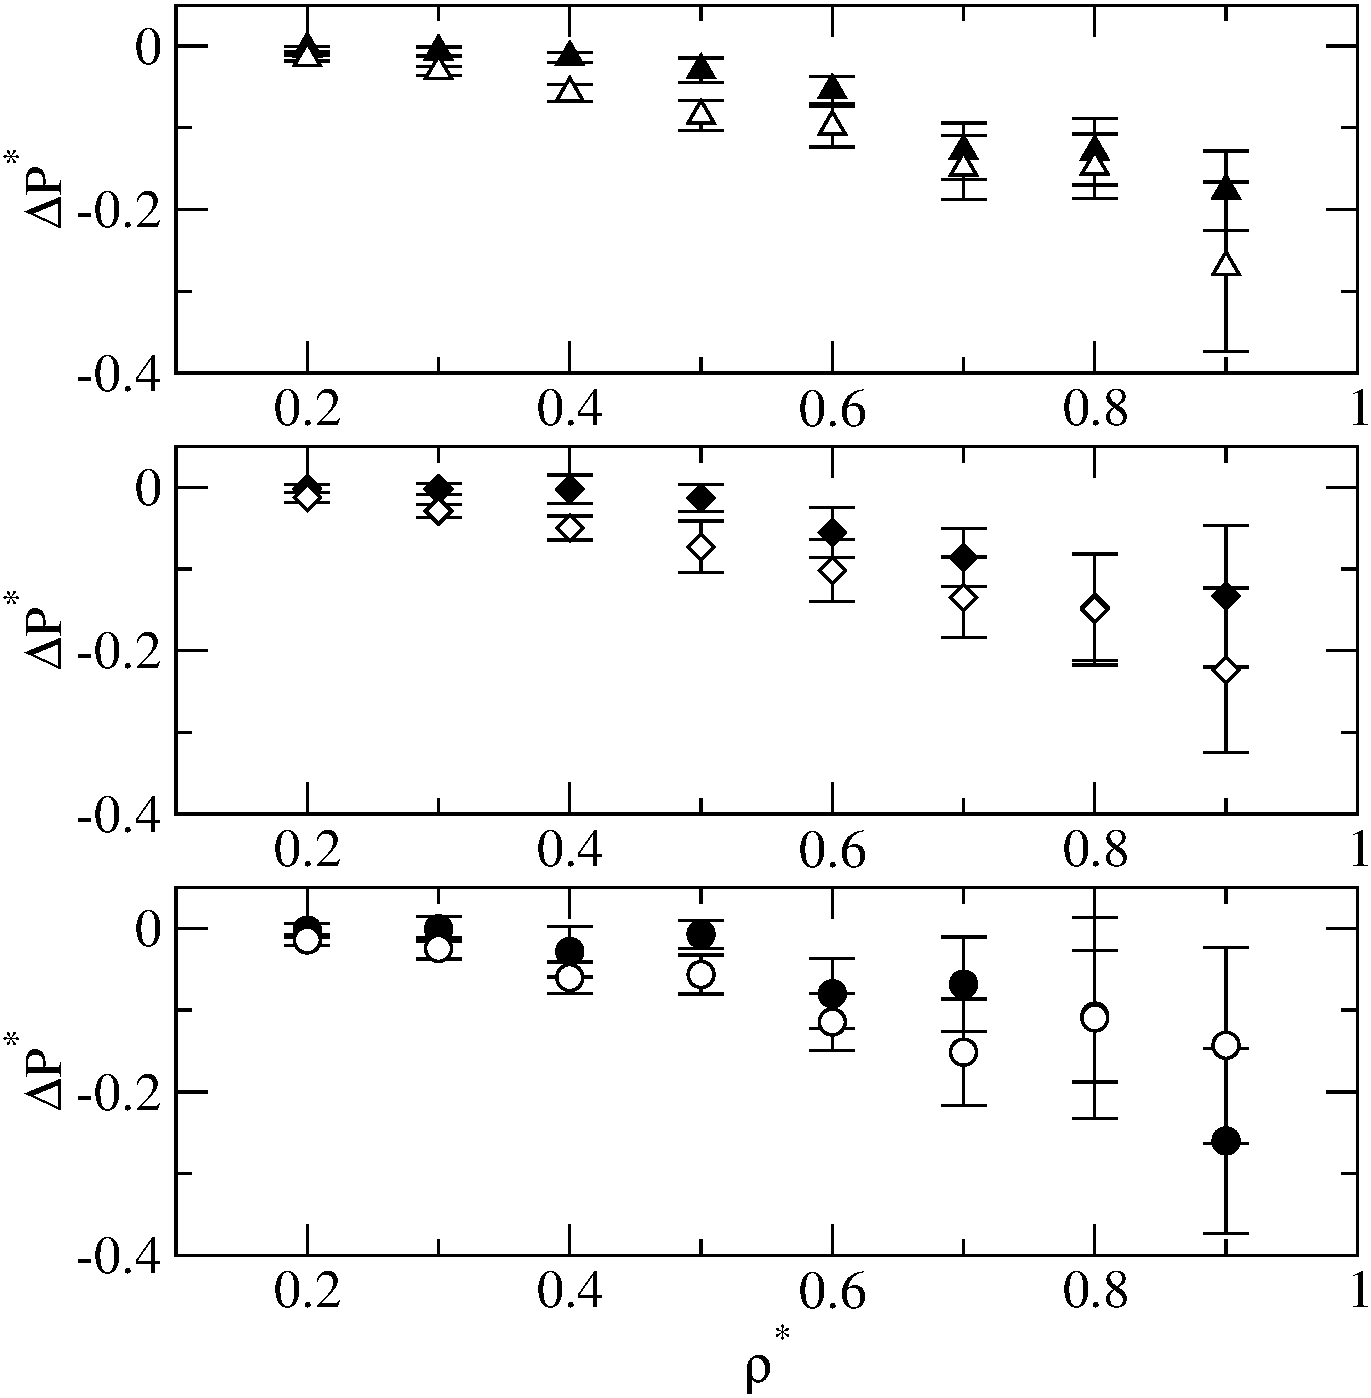
\includegraphics[clip,scale=0.45]{figures/TempP} 
    \caption[Temperature comparison of pressure between
    previous steps and this dissertations steps]
    {Temperature comparison of error in pressure obtained from
      Chapela \textit{et al.} steps (filled), and this dissertation's
      steps (unfilled) at temperatures of $T^*=1.5$ (triangle, top),
      $T^*=3.0$ (diamond, middle) and $T^*=4.5$ (circle, bottom).}
    \label{fig:tempP}
  \end{center}
\end{figure}

The plot for pressure is shown in Fig.~\ref{fig:tempP}. Unlike the
potential energy there is no discernible trend in the data for
increasing temperature.  This should be the case as the steps were set
to ensure probability was the same in both discrete and continuous
potentials.  It was shown in Sec.~\ref{sec:eqProb} that this was
equivalent to setting the second virial coefficient the same, so the
pressure should be maintained more accurately than the energy.  

If any trend can be identified it would be that the error at high
density seems to be reducing with temperature.  This is unusual as the
higher order virial coefficients should become more important at high
temperature~\cite{Sun1996}. However, the error bars significantly
larger than those for potential energy so there is the possibility
this trend is simply statistical error.

\section{Summary}

Now that the techniques for setting the stepping parameters have been
investigated, the best method is outlined here.  The optimal method
for setting the step positions is to ensure that the magnitude of the
expected force is equal in each step interval.  The heights of the
steps should be set to ensure the probability and hence, the second
virial coefficient, of the continuous and discrete potentials are the
same.  The inner hard core should be set at a location that four
standard deviations of particles do not reach.

The steps created by this method are compared with those created by
Chapela \textit{et al.} in Fig.~\ref{fig:stepComp}.  The steps are
similar, both concentrate their steps at the core, though those of
Chapela \textit{et al.} are further in than those created by this
method.  The results produced by both methods are very similar
(see Fig.~\ref{fig:ChapelaComp}); however, the steps created using the
above method have the advantage of that they are automatic.

\begin{figure}[htp] 
  \begin{center}
    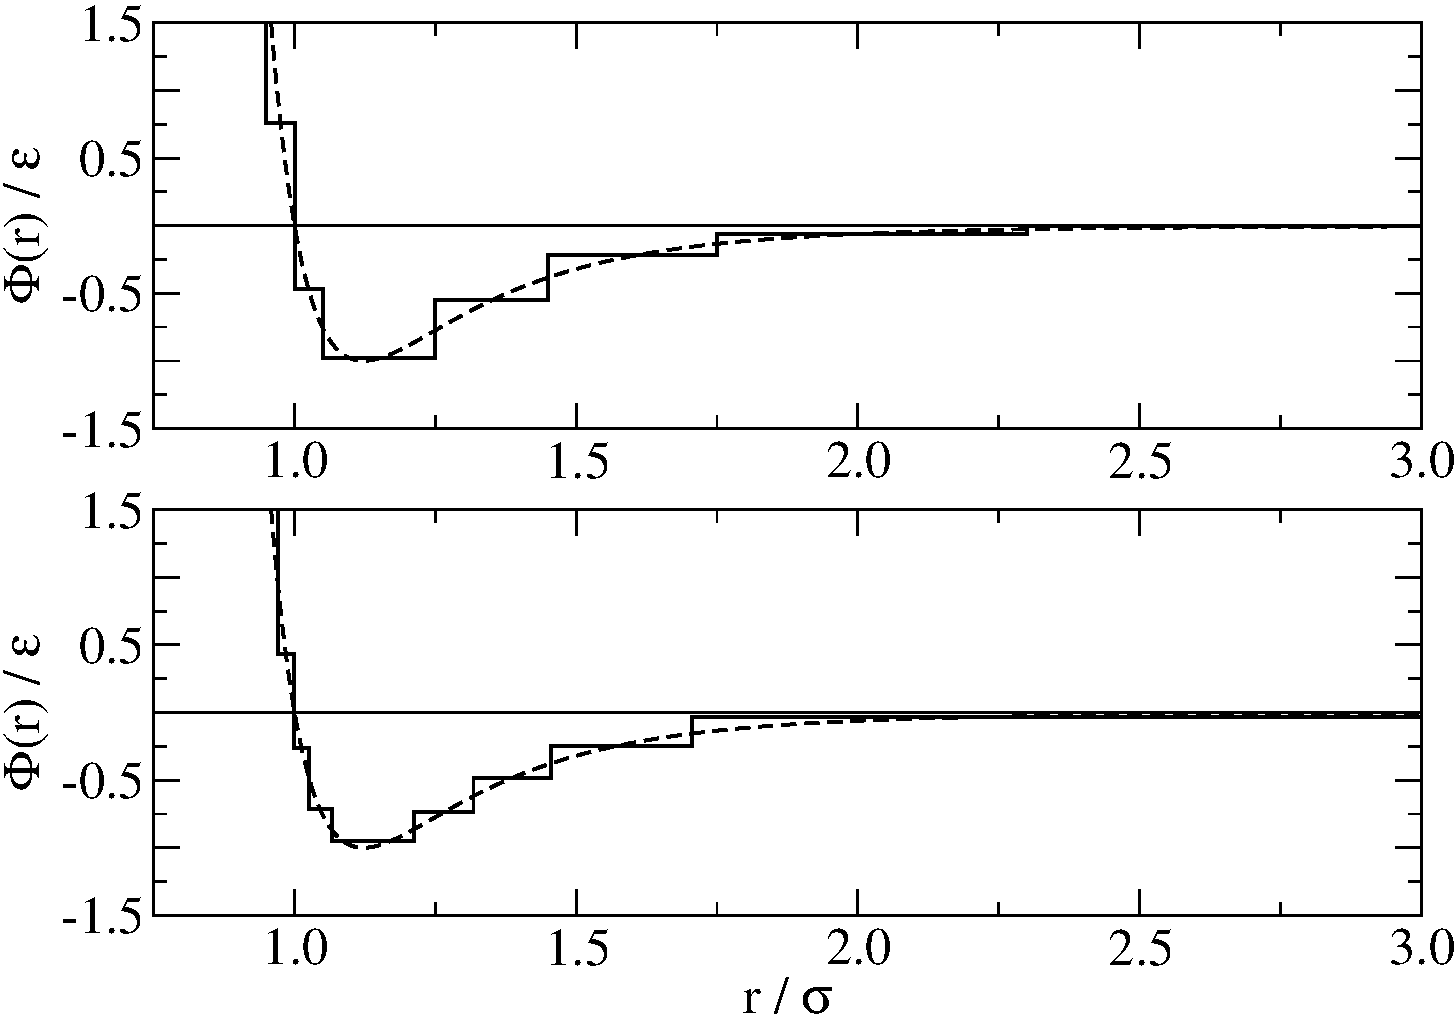
\includegraphics[clip,scale=0.45]{figures/stepComp} 
    \caption[Comparison of the steps created by Chapela \textit{et
      al.} and those created in this dissertation]
    {Comparison of the steps created by Chapela \textit{et al.} (top)
      and those created in this dissertation (bottom) at a temperature
      of $T^*=1.5$.}
    \label{fig:stepComp}
  \end{center}
\end{figure}


\printbibliography[heading=thesisChapterBib] 
\chapter{Conclusions and Future Work}
\section{Conclusions}
The aims of this dissertation were to create a working force-driven
and event-driven simulator, and to create a general method for
converting continuous to discrete potentials.  Both of these aims were
achieved in this dissertation.

A large part of this dissertation was the creation of the simulators
required to test the effectiveness of any conversion method.  Both the
simulators work correctly and include many of the optimisation
techniques (with the exception of a neighbour list in the event-driven
simulation) available to either simulation method.  This ensured that
a reasonable size system (864 particles, 1.5 million collisions) could
be simulated in a relatively short period of time (< 30 mins) on an
average desktop computer. Due to this a large number of comparisons,
each repeated a number of times, could be undertaken during the
timescale of this project.

A general method was created in this dissertation to convert a
continuous to discrete potential.  The method is outlined as
follows. The step positions were set to have equal magnitudes of the
expected force (see Sec.~\ref{sec:actionstep}). Meanwhile the step
energies were placed to ensure equal probabilities as the continuous
potential (Sec.~\ref{sec:eqProb}). The position of the hard core is
set at a position where four standard deviations of particles are
outside of that location.

This method successfully emulates the behaviour of the continuous
Lennard-Jones potential over a range of temperatures ($T^*=1.5-4.5$)
and densities ($\rho^*=0.2-0.9$).  It also gives comparable results to
the hand-made steps of Chapela \textit{et al.}~\cite{Chapela1989} and
has the major advantage that it can be implemented into the
simulator itself.  The event-driven simulator used in this
dissertation generated the steps using the outlined method at the
start of every simulation run.  This means that parameters such as the
number of steps can be changed easily and with no additional work.

With the automatic stepping procedure developed in this work, it is
possible to convert the large number of advanced continuous potentials
in the literature to discrete potentials.  This could allow accurate
predictions of thermodynamic properties for a wide range of fluids and
develop a deeper understanding of molecular interactions.

\section{Suggestions for Future Work}

While the stepping method presented in this dissertation is a
significant improvement over any existing method it would still
benefit from further work.

The most important problem of this method is that the core needs to
be manually hardened and its placement needs to be done separately.
Ideally, these should be taken into account by the methods for setting
set positions and heights.  Therefore although this method produces
very similar results to continuous potentials, there is still room for
improvement in both the step positioning and determining the heights
of the steps.  

If a radial distribution function generated from a force-driven
simulation could be implemented into the method, the validity of the
positioning and height determining methods could be verified.  Both of
these methods implicitly assume that the RDF is one, so the inclusion
of the RDF should give improved results.

While ten steps were used to model the continuous potential in this
study, this was done purely so a comparison could be made to Chapela
\textit{et al.}.  An investigation could also be carried out to find
the optimal number of steps; clearly more steps would model the
continuous potential better, but the increase in computational cost
required for this increase could be studied.

The aim of this general stepping method is that it is supposed to be
applicable to any potential.  In this dissertation, it was only
compared to Lennard-Jones potential during the method's development;
however, it should compared against a wide range of alternative
continuous potentials (such as CHARMM~\cite{MacKerell1998}) to check
whether it succeeds at this aim.
\printbibliography[heading=thesisChapterBib] 
\appendix
\chapter{Derivation of Collision Dynamics for Stepped Potentials }
\label{app:derivation}
Considering a collision between particles $i$ and $j$, each with mass,
$m$ with a step energy difference of $\Delta \Phi$, the conservation of
momentum is shown in Eq.~\eqref{eq:consMom}. Here the prime
indicates post-collision values.

\begin{equation}
\label{eq:consMom}
m\mathbf{v}_i + m\mathbf{v}_j = m\mathbf{v}'_i + m\mathbf{v}'_j
\end{equation}

The momentum change of each particle must occur along the separation
vector between the two particles, which can be expressed by:

\begin{equation}
  \label{eq:defA}
  m\mathbf{v}_i - m\mathbf{v}'_i = -(m\mathbf{v}_j - m\mathbf{v}'_j) 
  = -A\mathbf{\hat{r}}_{ij}
\end{equation}
where $A$ is an arbitrary coefficient.

Energy must also be conserved in the system so Eq.~\eqref{eq:constE}
must also apply.  This can be rewritten to Eqs.~\eqref{eq:constE1} and
\eqref{eq:constE2}

\begin{equation}
  \label{eq:constE}
  \frac{1}{2}mv_i^2 + \frac{1}{2}mv_j^2 =
  \frac{1}{2}m{v'_i}^2 + \frac{1}{2}m{v'_j}^2 + \Delta \Phi
\end{equation}

\begin{equation}
  \label{eq:constE1}
  v_i^2 - {v'_i}^2 +
  v_j^2 - {v'_j}^2 - \frac{2}{m}\Delta \Phi = 0
\end{equation}

\begin{equation}
  \label{eq:constE2}
  (\mathbf{v}_i - \mathbf{v}'_i)\cdot(\mathbf{v}_i + \mathbf{v}'_i) +
  (\mathbf{v}_j - \mathbf{v}'_j)\cdot(\mathbf{v}_j + \mathbf{v}'_j) -
  \frac{2}{m}\Delta \Phi = 0
\end{equation}

Equation \eqref{eq:defA} can now be substituted into
Eq.~\eqref{eq:constE2} to give Eq.~\eqref{eq:eq1}.

\begin{equation}
  \label{eq:eq1}
  \frac{A}{m}\mathbf{\hat{r}}_{ij} (\mathbf{v}_j - \mathbf{v}_i 
  + \mathbf{v}'_j - \mathbf{v}'_i) - \frac{2}{m}\Delta \Phi = 0
\end{equation}

Equation \eqref{eq:defA} and the definition of the separation velocity
vector ($\mathbf{v}_{ij} = \mathbf{v}_i - \mathbf{v}_j$) can be
substituted into Eq.~\eqref{eq:eq1} to give Eq.~\eqref{eq:eq2}.

\begin{equation}
  \label{eq:eq2}
  -\frac{A^2}{m}
  -A\mathbf{\hat{r}}_{ij}\cdot\mathbf{v}_{ij} - \Delta \Phi = 0
\end{equation}

This is a quadratic equation in terms of $A$ therefore it's roots must
be given by equation:

\begin{equation}
  \label{eq:devQuadratic}
  A = -\frac{m}{2}\left((\mathbf{v}_{ij}\cdot\mathbf{\hat{r}}_{ij}) \pm
  \sqrt{(\mathbf{v}_{ij}\cdot\mathbf{\hat{r}}_{ij})^2 - \frac{4}{m}\Delta \Phi}\right)
\end{equation}  

From Eq.~\eqref{eq:defA}, the change in velocity of each particle
is given in Eqs.~\eqref{eq:deltaV}

\begin{subequations}
  \label{eq:deltaV}
  \begin{align}
    \Delta\mathbf{v}_i &= \frac{A}{m} \mathbf{\hat{r}}_{ij} \\
    \Delta\mathbf{v}_j &= -\frac{A}{m}\mathbf{\hat{r}}_{ij}    
  \end{align}
\end{subequations}

\printbibliography[heading=thesisChapterBib] 
 
\end{document}

%%%%TAYLOR SERIES FOR GEAR'S ALGORITHM%%%% %\begin{equation} 
%\begin{aligned}
%\vec{r}(t+\Delta t) &= \vec{r}(t) + \vec{v}(t) \Delta t 
% +\frac{1}{2}\vec{a}(t)\Delta t^2 + \frac{1}{3!}\vec{b}(t)\Delta t^3 
% +\frac{1}{4!}\vec{c}(t)\Delta t^4 + \frac{1}{5!}\vec{d}(t)\Delta t^5 \\
%\vec{v}(t+\Delta t) &= \vec{v}(t) \Delta t + \vec{a}(t)\Delta t^2 
% +\frac{1}{2}\vec{b}(t)\Delta t^3 + \frac{1}{3!}\vec{c}(t)\Delta t^4 +
%\frac{1}{4!}\vec{d}(t)\Delta t^5 \\ %\vec{a}(t+\Delta t) &= \vec{a}(t)\Delta
%t^2+ \vec{b}(t)\Delta t^3 % + \frac{1}{2!}\vec{c}(t)\Delta t^4 +
%\frac{1}{3!}\vec{d}(t)\Delta t^5 \\ %\vec{b}(t+\Delta t) &= \vec{b}(t)\Delta
%t^3+ \vec{c}(t)\Delta t^4 % + \frac{1}{2!}\vec{d}(t)\Delta t^5 \\
%\vec{c}(t+\Deltat) &= \vec{c}(t)\Delta t^4 + \vec{d}(t)\Delta t^5 \\
%\vec{d}(t+\Delta t) &=
%\vec{d}(t)\Delta t^5 \\ %\end{aligned} %\end{equation}
